\pdfoutput=1
%% ****** Start of file apstemplate.tex ****** %
%%
%%
%% This file is part of the APS files in the REVTeX 4 distribution.
%% Version 4.1r of REVTeX, August 2010
%%
%%
%% Copyright (c) 2001, 2009, 2010 The American Physical Society.
%%
%% See the REVTeX 4 README file for restrictions and more information.
%%
%
% This is a template for producing manuscripts for use with REVTEX 4.0
% Copy this file to another name and then work on that file.
% That way, you always have this original template file to use.
%
% Group addresses by affiliation; use superscriptaddress for long
% author lists, or if there are many overlapping affiliations.
% For Phys. Rev. appearance, change preprint to twocolumn.
% Choose pra, prb, prc, prd, pre, prl, prstab, prstper, or rmp for journal
% Add 'draft' option to mark overfull boxes with black boxes
% Add 'showpacs' option to make PACS codes appear
% Add 'showkeys' option to make keywords appear
\documentclass[aps,prd,twocolumn,superscriptaddress,preprintnumbers,floatfix,nofootinbib]{revtex4-2}
%\documentclass[aps,prl,preprint,superscriptaddress]{revtex4-1}
%\documentclass[aps,prl,reprint,groupedaddress]{revtex4-1}

\usepackage{graphicx}
\usepackage{amsmath}
%\usepackage{mdwlist}
\usepackage[caption=false]{subfig}
\usepackage{siunitx}
\usepackage{placeins}
\usepackage{color}
\usepackage{standalone}
\usepackage{dcolumn}
\usepackage{tensor}
\usepackage{bm}
%\usepackage{MnSymbol}
\usepackage{microtype}
\usepackage{etoolbox}
\usepackage{amssymb}
\usepackage{mathrsfs}
\usepackage{accents}
\usepackage[normalem]{ulem}
\usepackage[dvipsnames]{xcolor}
\usepackage[colorlinks,urlcolor=NavyBlue,citecolor=NavyBlue,linkcolor=NavyBlue,pdfusetitle]{hyperref}
\usepackage[all]{hypcap}
\usepackage[inline]{enumitem}
\usepackage[utf8]{inputenc}
\usepackage{csquotes}
\usepackage{array}
\usepackage{booktabs}
\usepackage[T1]{fontenc}

\newcommand{\ts}{\textsuperscript}

\newcommand{\beq}{\begin{equation}}
\newcommand{\eeq}{\end{equation}}

\newcommand{\nn}{\nonumber}

\newcommand*{\eq}[1]{Eq.~\eqref{eq:#1}}
\newcommand*{\fig}[1]{Fig.~\ref{fig:#1}}
\newcommand*{\sect}[1]{Sec.~\ref{sec:#1}}

\newcommand{\boldmu}{\boldsymbol{\mu}}
\newcommand{\boldn}{\mathbf{n}}
\newcommand{\boldd}{\mathbf{d}}
\newcommand{\bolds}{\mathbf{s}}
\newcommand{\boldSigma}{\boldsymbol{\Sigma}}

\newcommand{\area}{\mathcal{A}}

%% Try to control orphans, widows, and extra whitespace
%\widowpenalty=10000
%\clubpenalty=10000
%\raggedbottom
\interfootnotelinepenalty=3000

%% Enable/disable comments
\newtoggle{commentsoff}
\togglefalse{commentsoff}
%\toggletrue{commentsoff}

% Check for command-line option to turn comments off
% https://tex.stackexchange.com/questions/1492/passing-parameters-to-a-document
\ifdefined\nocomments
    \toggletrue{commentsoff}
\fi

\iftoggle{commentsoff}{
  \newcommand*{\mi}[1]{}
  \newcommand*{\mg}[1]{}
  \newcommand*{\wf}[1]{}
  \newcommand*{\comment}[1]{}
  \newcommand*{\suggest}[3]{#2}
  \newcommand*{\todo}[1]{}
  \newcommand*{\warn}[1]{}
  \newcommand*{\red}[1]{#1}
  \newcommand*{\blue}[1]{#1}
  \newcommand{\cn}{}
  \newcommand*{\commentmark}[1]{}
}{
  \newcommand*{\mi}[1]{{\color{magenta} [{\bf MAX}: #1]}}
  \newcommand*{\wf}[1]{\textcolor{green}{\textbf{WILL}: #1}}
  \newcommand*{\suggest}[3]{\textcolor{Purple}{\textbf{#3} \sout{#1} #2}}
  \newcommand*{\comment}[1]{{\color{blue} [{\bf NOTE}: #1]}}
  \newcommand*{\warn}[1]{{\color{red} [{\bf WARNING}: #1]}}
  \newcommand*{\todo}[1]{{\color{red} [{\bf TODO}: #1]}}
  \newcommand*{\red}[1]{{\color{purple} #1}}
  \newcommand*{\blue}[1]{{\color{blue} #1}}
  \newcommand{\cn}{\blue{\bf [cn]}}
}

\graphicspath{{./fig/}}

\newcommand{\dcc}{LIGO-PXXXXXXX}

% NOTATION MACROS
\newcommand{\infd}{\mathrm{d}}
\newcommand{\white}{\bar}

\newcommand{\snropt}{\mathrm{SNR}}
\newcommand{\snrmf}{\mathrm{SNR}_{\rm mf}}
\newcommand{\cov}{C}
\newcommand{\acf}{\rho}
\newcommand{\nmode}{D}

\begin{document}

% Use the \preprint command to place your local institutional report
% number in the upper righthand corner of the title page in preprint mode.
% Multiple \preprint commands are allowed.
% Use the 'preprintnumbers' class option to override journal defaults
% to display numbers if necessary
% \preprint{\dcc}

%Title of paper
\title{Parametrizing gravitational-wave polarizations}

\author{Maximiliano Isi}
\email[]{misi@flatironinstitute.org}
%\thanks{NHFP Einstein fellow}
%\homepage[]{Your web page}
%\thanks{}
%\altaffiliation{}
% \affiliation{
% LIGO Laboratory, Massachusetts Institute of Technology, Cambridge, Massachusetts 02139, USA
% }%
\affiliation{Center for Computational Astrophysics, Flatiron Institute, 162 5th Ave, New York, NY 10010}

% Because hyperref only gets the *last* author, we need to be explicit.
\hypersetup{pdfauthor={Isi}}

\date{\today}

\begin{abstract}
Amazing!
\end{abstract}

\maketitle

% \tableofcontents

\section{Introduction}
\label{sec:intro}

It is useful to parametrize gravitational-wave (GW) polarizations in different ways.
Here I outline some useful alternatives and show how they are related.
It is important to understand the priors implied by the choice of parametrization through the corresponding Jacobians.

The goal of this note is twofold.
First, pedagogical, in reviewing different polarization conventions and their relation.
Second, technical, in providing explicit expressions for Jacobians relating different polarization parametrizations, ready for implementation in parameter estimation codes or similar applications.

This note is geared towards observers, or theorists interested in drawing connections to observation.
As such, it aims for concreteness, rather than comprehensiveness; it does not cover formal aspects of the frameworks connecting to the mathematical structure of general relativity and multipole expansions therein.
References are provided when such links are possible.

\section{Polarization primer}

\subsection{Linear basis}

In GR, there exist two propagating gravitational degrees of freedom, corresponding to two independent GW polarizations (e.g., \cite{Thorne1983,Thorne:1987af,Poisson2014,BT}).
At any given time, their local effect can be encoded in a driving matrix $h_{ij}$ representing the transverse-traceless part of the metric perturbation, also known as the \emph{gravitational-wave field}.
In a Cartesian frame with $z$-axis along the direction of propagation, we can write this matrix as
\beq \label{eq:hij}
(h_{ij}) = \begin{pmatrix}
h_+ & h_\times  & 0 \\
h_\times  & - h_+ & 0  \\
0 & 0 & 0
\end{pmatrix} ,
\eeq
where the plus ($+$) and cross ($\times$) polarization functions, $h_{+/\times}$, depend implicitly on the retarded time, $t - R/c$, in a way determined by the source dynamics and by the (luminosity) distance $R$ to the source.

\begin{figure}
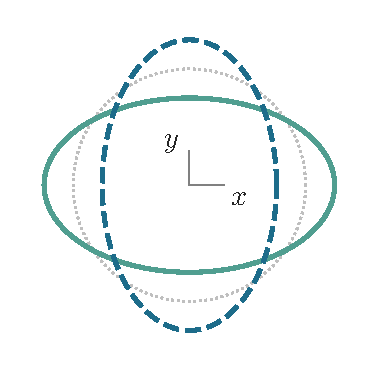
\includegraphics[width=0.4\columnwidth]{pol_ring_plus}
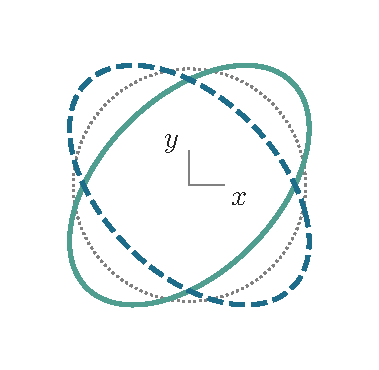
\includegraphics[width=0.4\columnwidth]{pol_ring_cross}
\caption{Effect of plus (left) and cross (right) polarizations on a small, freely falling ring of particles. The wave propagates in the $z$ direction, perpendicular to the page. The effect is illustrated half a period apart (solid vs dashed); the unperturbed ring is also shown for reference (thin dotted line).
}
\label{fig:rings}
\end{figure}

It can be useful to rewrite \eq{hij} as $h_{ij} = h_+ e^+_{ij} + h_\times e^\times_{ij}$, in terms of the $e^{+/\times}_{ij}$ polarization basis tensors given by
\begin{subequations} \label{eq:lin}
\begin{align}
e^+_{ij} &\equiv \hat{x}_i \hat{x}_j - \hat{x}_i \hat{x}_j \, ,\\
e^\times_{ij} &\equiv \hat{x}_i \hat{y}_j + \hat{x}_i \hat{y}_j\, ,
\end{align}
\end{subequations}
where $\hat{x}$ and $\hat{y}$ are arbitrary orthonormal vectors that, with $\hat{z}$, form a right-handed orthonormal basis; we will call this the \emph{wave frame}.
Since this frame is constructed to have $\hat{z}$ aligned with the wavevector $\vec{k}$ (i.e., $\hat{z} = \hat{k} \equiv \vec{k}/|k|$), the polarization tensors are implicit functions of the wave propagation direction $\hat{k}$, or, equivalently, the source sky location $\hat{n} = -\hat{k}$.
For a given $\hat{k}$, it is easy to check that these tensors are orthogonal such that $e^p_{ij} e^{p'ij}=2\delta^{pp'}$ for $p,p'$ in $\{+,\times\}$.
% Generic metric theories beyond GR generally predict up to four additional polarizations, which we briefly address in Sec.~\ref{sec:nongr}.

We will refer to plus and cross jointly as the \emph{linear} polarization basis.
Their physical interpretation is best illustrated by their instantaneous effect on a freely-falling ring of particles, as shown in Fig.~\ref{fig:rings}.
Other polarization bases can be constructed, as we will see below, but the linear polarizations are generally the most convenient for expressing measurements.

In the small-antenna limit, the signal induced by a passing GW on a given detector can be written as the projection
\beq \label{eq:h}
h(t) \equiv D^{ij} h_{ij} = F_+ h_+ + F_\times h_\times\, 
\eeq
with antenna patterns $F_{+/\times} \equiv D^{ij} e^{+/\times}_{ij}$ defined in terms of a detector tensor $D_{ij}$ that encodes the geometry of the measurement.
For a differential-arm detector like LIGO with arms pointing along unit vectors $\hat{X}$ and $\hat{Y}$, this is just $D_{ij} = (\hat{X}_i \hat{X}_j - \hat{Y}_i \hat{Y}_j)/2$.%
\footnote{These expressions are valid in the local Lorentz frame of the detector, so we can raise and lower indices with the flat metric.}
In this limit, the antenna patterns are thus purely geometric factors that encode the relative orientations of the detector and wave frames, as defined by $\{\hat{X},\, \hat{Y},\, \hat{Z}\}$ and $\{\hat{x},\, \hat{y},\, \hat{z}\}$ respectively.

% Equation \eqref{eq:hij} presumes a specific choice of wave frame orientation that defines the basis in which the $h_{ij}$ components are written.
% Although \eq{hij} requires that $\hat{z}$ be parallel to the (spatial) wave vector $\vec{k}$, there is no a priori restriction on the orientation of the $x$ and $y$ axes within the plane perpendicular to $\vec{k}$.
% %This freedom is usually encapsulated in the choice of an arbitrary \emph{polarization angle} $\psi$, defined with respect to some convenient reference (e.g., the celestial equator \cite{LALSuite:wave}).
% With some trigonometry, it is straightforward to show that a rotation of the frame by some angle $\Delta \psi$ around $z$ leaves the form of \eq{hij} unchanged after redefining
% \begin{subequations} \label{eq:htransf}
% \begin{align}
% h_+ &\rightarrow h_+' = h_+ \cos 2\Delta \psi - h_\times \sin 2\Delta\psi \, , \\
% h_\times &\rightarrow h_\times' = h_\times \cos 2\Delta \psi + h_+ \sin 2\Delta\psi \, .
% \end{align}
% \end{subequations}
% This reveals the fact that $h_+$ and $h_\times$ are nothing but the two components of a tensor field with spin-weight $|s|=2$, and the two polarizations are only defined up to an arbitrary rotation.
% (We return to this point in Sec.~\ref{sec:pol}.)

After fixing the frame orientation, any plane GW may be expressed in terms of the Fourier components of its polarization amplitudes as
\begin{align}
\label{eq:planewave}
h_{ij}(t,\vec{x}) &= \frac{1}{2\pi}\int_{-\infty}^{+\infty} \tilde{h}_{ij}(\omega, \hat{k})\, e^{i\omega \left(\frac{\hat{k}\cdot\vec{x}}{c}-t\right)} \infd \omega \\
&= \frac{1}{2\pi} \sum_{p=+,\times} \int_{-\infty}^{+\infty} \tilde{h}_p(\omega)\, e^p_{ij}(\hat{k})\, e^{i\omega \left(\frac{\hat{k}\cdot\vec{x}}{c}-t\right)} \infd \omega \nonumber
\end{align}
where the sum is over linear polarization states ($+,\times$) defined in some wave frame attached to the propagation direction $\hat{k}$,%
\footnote{More broadly, the strain value at any point in spacetime may be expressed with full generality as a superposition of these planewaves
% $h_{ij}(t,\vec{x}) = \int_{\mathcal{S}^2} \int_{-\infty}^{+\infty} \tilde{h}_p(\omega, \hat{k})\, e^p_{ij}(\hat{k})
% \exp\left[{i\omega \left(\hat{k}\cdot\vec{x}/c-t\right)}\right] \infd \omega \infd \hat{k}$
by integrating over all directions of propagation.}
and we obtained the second line using the fact that the $e^{+/\times}_{ij}$ are real valued.
Equation \eqref{eq:planewave} implicitly defines the complex-valued Fourier polarization functions $\tilde{h}_p(\omega)$ to correspond to the time-domain polarizations at the spatial origin, $h_p(t) \equiv h_p(t, \vec{x}=0)$, by
\beq \label{eq:ft}
\tilde{h}_p(\omega) \equiv \int_{-\infty}^{+\infty} h_p(t)\, e^{i\omega t} \infd t \, ,
\eeq
establishing our convention for the Fourier transform.

Since $h_{ij}$ is real valued, the Fourier strain must  satisfy the complex-conjugate symmetry $\tilde{h}_{ij}(-\omega, \hat{k}) = \tilde{h}_{ij}^*(\omega,\hat{k})$, where the asterisk indicates complex conjugation.
For the linear polarizations, this reduces to
\beq \label{eq:sym_linear}
\tilde{h}_{+/\times}(\omega) = \tilde{h}_{+/\times}^*(-\omega)\, ,
\eeq
because the linear basis tensors are themselves real valued.
As usual, then, the positive and negative frequencies must be considered as inseparable contributions to a single Fourier mode.
The existence of this symmetry reveals a redundancy in the description that we can exploit to write Eq.~\eqref{eq:planewave} more concisely.

\begin{figure*}
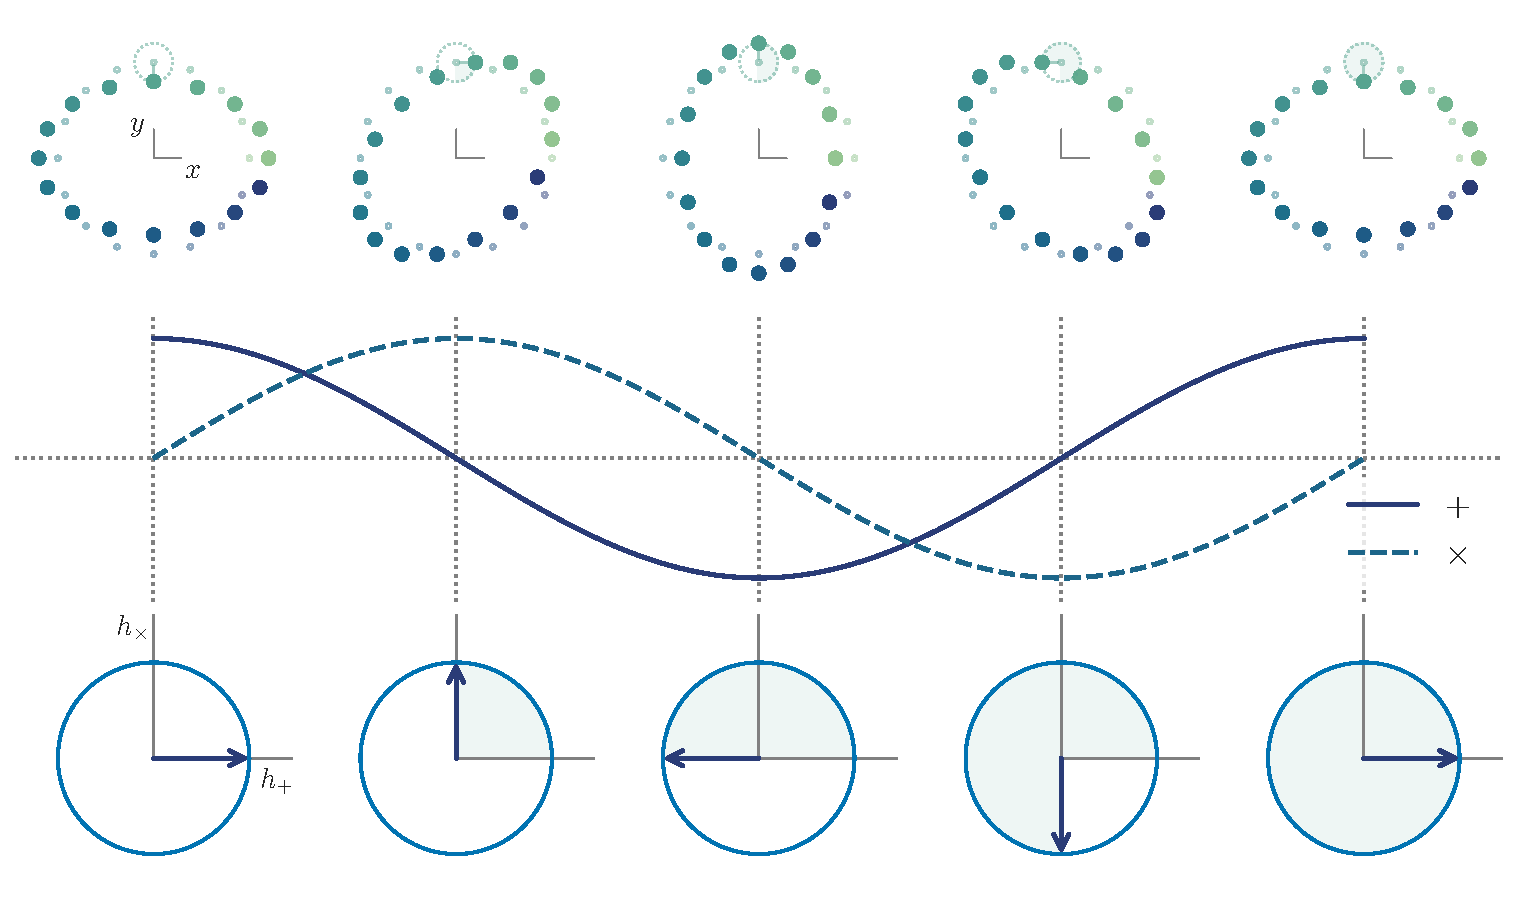
\includegraphics[width=0.8\textwidth]{pol_diagram_circ}
\caption{A right-handed, circularly polarized GW as a function of time (left to right) over a period. \emph{Top:} as the wave propagates out of the page, it deforms a freely falling ring of particles (colored dots) into an ellipsoidal pattern, which rotates counterclockwise with time; each individual particle is pushed in a circle around its original location, i.e., the location it would have had in absence of the wave (small empty circles).
\emph{Middle:} amplitudes of the plus (solid) and cross (dashed) linear polarizations making up the wave as a function of time; the plus polarization is $\pi/2$ radians ahead of the cross polarization.
\emph{Bottom:} representation of the polarization state as a Jones vector in the $+$ and $\times$ space; the phasor rotates counterclockwise in a circle.
Reversing the direction of time by reading this diagram right-to-left gives the effect of a left-handed circularly polarized wave.
}
\label{fig:pol_diagram_circ}
\end{figure*}

\subsection{Circular basis}

First, instead of the linear plus and cross polarizations above, we could equivalently work with the associated \emph{circular} right-handed (R) and left-handed (L) modes.
%, which are eigenstates of the helicity operator.
These are defined in the Fourier domain by the complex-valued basis tensors
\beq \label{eq:circ}
e^{R/L}_{ij} \equiv \frac{1}{\sqrt{2}} \left(e^+_{ij} \pm i e^\times_{ij} \right) ,
\eeq
with the plus (minus) sign corresponding to R (L).
These tensors are also orthogonal and normalized similarly to $e^{+/\times}_{ij}$ such that $(e^{p'ij})^* e^p_{ij} = 2 \delta^{pp'}$ for $p,p'$ in $\{R,L\}$.

To understand the physical significance of the circular polarizations,
% consider an individual Fourier mode of frequency $\omega>0$ propagating in the positive-$z$ direction,
% \beq
% h_{ij}(t,z; \omega) = \Re \left\{ \tilde{H}_{ij} \exp[ i \omega (z/c - \omega t)]\right\},
% \eeq
% for some time and location independent (and complex-valued) amplitude tensor $\tilde{H}_{ij}$.
consider a purely R-polarized monochromatic mode $h^R_{ij}$ with frequency $\omega > 0$, unit amplitude and zero phase offset; at the spatial origin ($\vec{x}=0$), the time-domain strain from such a mode will be given by
\begin{align} \label{eq:circ_example}
h_{ij}^R(t;\omega) &= \Re \left[ e^R_{ij}\, \exp(-i\omega t) \right] \nonumber\\
%&= \frac{1}{\sqrt{2}} \Re \left[\left(e^+_{ij} + i e^\times_{ij}\right) \exp(-i\omega t) \right] \nonumber\\
&= \frac{1}{\sqrt{2}} \left( e^+_{ij} \cos \omega t + e^\times_{ij} \sin \omega t \right) ,
\end{align}
using the definition from Eq.~\eqref{eq:circ}.
In the 2D Cartesian space defined by the linear polarization amplitudes, i.e. $\left(h_+, h_\times\right)$, this defines a circle, around which the \emph{phasor} encoding the state of the wave rotates counterclockwise (for $\omega > 0$).
This means that, at any given time, the wave will have a unit total amplitude (i.e., $h^2_+ + h^2_\times=1$) and the cross polarization will \emph{lag behind} the plus polarization by $\pi/2$ radians in phase.
%
Consequently, a purely R-polarized wave will deform a ring of freely-falling particles into an elliptical pattern that is seen to rotate counter-clockwise when looking towards the source (Fig.~\ref{fig:pol_diagram_circ}), i.e., it follows the right-hand rule relative to the direction of propagation (pointing away from the source).
The opposite will be true for purely L-polarized waves, which will result in a clockwise-rotating ellipse.
%\footnote{If we let $\omega < 0$ then the roles of R and L would flip, indicating these states are invariant under parity-time transformations.}
This assignment of the ``right'' and ``left'' labels is known as the ``source based'' handedness convention.

The orthogonality and completeness of the tensors in Eq.~\eqref{eq:circ} mean that we can rewrite Eq.~\eqref{eq:planewave} in terms of the circular polarizations without loss of generality as the sum
\beq \label{eq:planewave_circ}
h_{ij}(t,\vec{x}) 
= \frac{1}{2\pi} \sum_{p=R,L} \int_{-\infty}^{+\infty} \tilde{h}_p(\omega)\, e^p_{ij}(\hat{k})\, e^{i\omega \left(\frac{\hat{k}\cdot\vec{x}}{c}-t\right)} \infd \omega \, ,
\eeq
where $\tilde{h}_{R/L}$ and $e^{R/L}_{ij}$ have replaced their $+/\times$ counterparts.
As is straightforward to show from Eq.~\eqref{eq:circ}, the circular and linear polarization Fourier amplitudes are related by
\begin{align} \label{eq:circ_amps}
\tilde{h}_{R/L} = \frac{1}{\sqrt{2}} \left(\tilde{h}_+ \mp i\tilde{h}_\times \right) ,
\end{align}
with the minus (plus) sign for R (L).
Based on this, the complex-conjugate condition of Eq.~\eqref{eq:sym_linear} implies that
\beq \label{eq:sym_circular}
\tilde{h}_R(\omega) = \tilde{h}_L^*(-\omega) \, ,
\eeq
which again manifests the redundancy in Eq.~\eqref{eq:planewave_circ}, as in Eq.~\eqref{eq:planewave}.
It also reveals that R and L switch roles for $\omega \to - \omega$, as we anticipated below Eq.~\eqref{eq:circ_example}, indicating that these states are invariant under parity-time reversals.


\subsection{Elliptical basis}
\label{sec:ellip}

%\subsubsection{Complex strain}

Next, it is convenient to encode the two linear GW polarizations as quadratures of a single complex-valued scalar field, $h_+ - i h_\times$, in the time domain.
This complex number provides an alternative representation of the $\left(h_+, h_\times\right)$ phasor introduced in the previous section (see bottom panel of Fig.~\ref{fig:pol_diagram_circ}).
If this quantity, the \emph{complex strain}, is purely real (imaginary), then the wave is purely plus (cross) polarized.
In those same terms, a unit-amplitude circularly-polarized mode like the one in \eq{circ_example} can be expressed simply as $h_+ - i h_\times = \exp(\mp i \omega t)/\sqrt{2}$, with the minus (plus) sign in the exponent corresponding to R (L) for $\omega > 0$.%
\footnote{The choice of sign in the definition of the complex strain as $h_+ - ih_\times$ matches the convention of the Fourier transform in Eq.~\eqref{eq:ft} in order to make it so that $\exp(-i|\omega| t)$ encodes a right-handed mode as defined in the source-based convention.}

Using this fact, an economic way of expressing the information in Eq.~\eqref{eq:planewave} for any given direction of propagation $\hat{k}$ is to write the time-domain complex strain at the spatial origin ($\vec{x}=0$) as a Fourier integral of the form
\begin{align} \label{eq:hcomp_fd}
h_+ - i h_\times = \frac{1}{2\pi} \int_{-\infty}^{+\infty} \tilde{H}(\omega)\, e^{-i \omega t} \,\infd \omega \, ,
\end{align}
where the complex-valued Fourier amplitudes are defined by $\tilde{H}(\omega) \equiv \int (h_+ - i h_\times) \exp(i\omega t)\, \infd t = \tilde{h}_+(\omega) - i \tilde{h}_\times(\omega)$, following our Fourier transform convention in Eq.~\eqref{eq:ft}.
Unlike in Eq.~\eqref{eq:planewave}, it is clear that these Fourier amplitudes will not generally satisfy the symmetry $\tilde{H}(-\omega) = \tilde{H}^*(\omega)$, since the quantity on the left hand side of Eq.~\eqref{eq:hcomp_fd} is not real-valued unless the wave is fully plus-polarized.

In fact, given the interpretation of $\exp(\pm i \omega t)$ discussed above, the positive (negative) frequency Fourier amplitudes in Eq.~\eqref{eq:hcomp_fd} must encode contributions from the R-polarized (L-polarized) portion of the waveform.
This becomes obvious if we note that, by Eq.~\eqref{eq:circ_amps} and the definition of $\tilde{H}$, it must be the case that $\tilde{H}(\omega) = \sqrt{2}\, \tilde{h}_R (\omega) = \sqrt{2} \tilde{h}_L^*(-\omega)$, the last equality being due to Eq.~\eqref{eq:sym_circular}.
We can leverage this to rewrite Eq.~\eqref{eq:hcomp_fd} as an integral restricted to positive frequencies,
\begin{equation} \label{eq:hcomp_fd_rl}
h_+ - i h_\times = \frac{1}{\sqrt{2\pi^2}} \int_{0}^{\infty} \left[ \tilde{h}_R(\omega)\, e^{-i \omega t} + \tilde{h}_L^*(\omega)\, e^{i \omega t}\right] \infd \omega \, .
\end{equation}
This expression carries the same information as Eq.~\eqref{eq:planewave} without any redundancies.

\begin{figure}
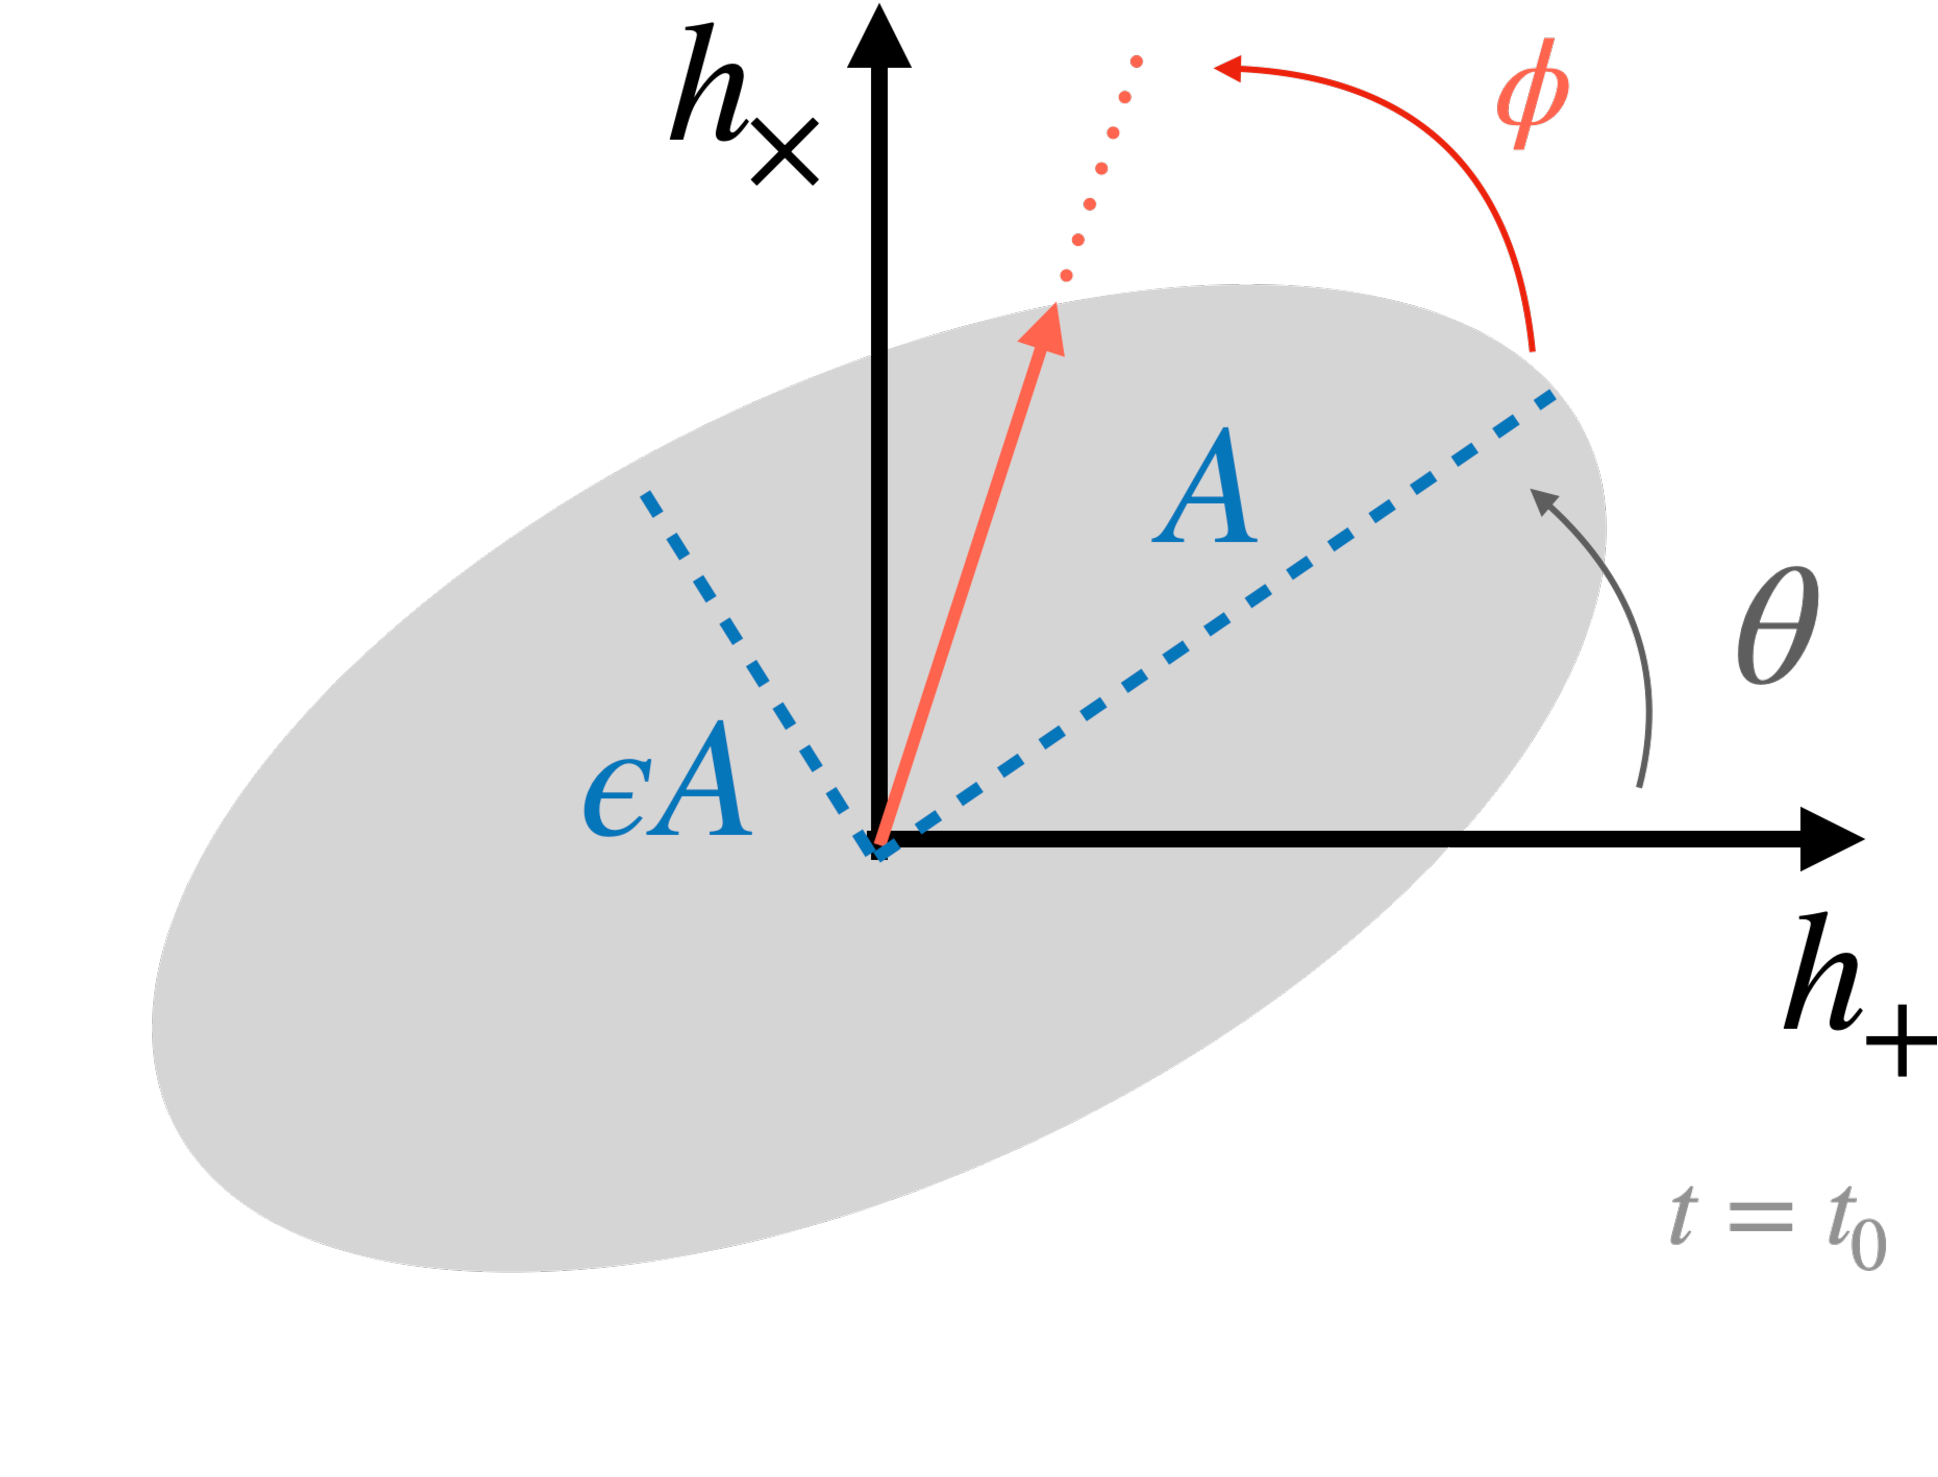
\includegraphics[width=0.6\columnwidth]{ellipse}
\caption{Polarization ellipse. At any given time, the phasor of an elliptically polarized signal lies on an ellipse with some instantaneous amplitude $A(t)$ and time-independent ellipticity $\epsilon$, with semimajor axis tilted by an angle $\theta$ with respect to the plus-polarization axis (abscissa); a second angle, $\phi \equiv \Phi(t=0)$, determines the initial location of the phasor within the ellipse. (Adapted from \cite{Isi:2021iql}.)}
\label{fig:ellipse}
\end{figure}

Equation \eqref{eq:hcomp_fd_rl} lends itself to a straightforward physical interpretation.
Any plane GW, with arbitrary time evolution and polarization state (including unpolarized states), can be expressed as a superposition of fully-polarized Fourier modes;
each such monochromatic mode of frequency $|\omega|$ is made up of two counterrotating circularly-polarized contributions (R and L, the two summands) that add up to a single elliptically polarized mode.
Such elliptical, or \emph{fully-polarized}, modes are thus of fundamental importance; we discuss their properties in detail below, beginning with modes of a definite frequency as they appear in \eq{hcomp_fd_rl}.

\section{Elliptical modes}
\label{sec:ellip}

\subsection{Monochromatic modes}
\label{sec:ellip:mono}

Elliptical GWs define an ellipse in the $\left(h_+, h_\times\right)$ phasor space.
We can see this explicitly for the Fourier modes in Eq.~\eqref{eq:hcomp_fd_rl} above by considering a monochromatic signal given by $\tilde{h}_{R/L}(\omega) = \pi\, \delta(\omega-\omega_0)\, C_{R/L} $,%
\footnote{The prefactor can be motivated by noting that $\tilde{h}_{R/L}(\omega) = 2\pi \delta(\omega - \omega_0) C_{R/L}/2 = \delta(f - f_0) C_{R/L} / 2$ implies that $C_{R/L}/2$ are amplitude densities with respect to the frequency $f \equiv \omega/2\pi$; the additional factor of $1/2$ normalizes the signal power such that $h_+^2 + h_\times^2 = 1$ for $|C_R|=1, |C_L|=0$ or $|C_R|=0, |C_L|=1$.}
isolating a single Fourier mode of frequency $\omega_0 >0$ and complex-valued amplitudes $\pi\, C_{R/L}$.
The result of the Fourier integral is then (relabeling $\omega_0 \to \omega$ after integration)
\begin{align} \label{eq:ellip_circ}
h_+ - i h_\times =\frac{1}{\sqrt{2}} \left( C_R\, e^{-i \omega t} + C^*_L\, e^{i\omega t}\right)\, ,
\end{align}
which can, without loss of generality, be refactored into
\begin{align}
h_+ - i h_\times = \frac{1}{2}A\left[ \left(1+\epsilon\right) e^{-i (\omega t - \phi_R)} + \left(1-\epsilon\right) e^{i (\omega t - \phi_L)} \right] .
\end{align}
% 
% refactor the integrand in Eq.~\eqref{eq:hcomp_fd_rl} as%
% \footnote{We factor $\sqrt{2}$ into the integrand so that, mirroring Eq.~\eqref{eq:ft}, the amplitude $A$ in this context is an amplitude spectral density with respect to the frequency $f \equiv \omega/(2\pi)$.}
% \begin{align}
% \sqrt{2} \left(\tilde{h}_R\, e^{-i \omega t} + \tilde{h}_L^*\, e^{i \omega t}\right) =\nonumber\\
% \frac{1}{2}A\left[ \left(1+\epsilon\right) e^{-i (\omega t - \phi_R)} + \left(1-\epsilon\right) e^{i (\omega t - \phi_L)} \right],
% \end{align}
In this expression, 
$A \equiv (|{C}_R| + |{C}_L| )/ \sqrt{2} \geq 0$ is the peak amplitude of the mode, $-1 \leq \epsilon = (|{C}_R| - |{C}_L|)/(|{C}_R| + |{C}_L|) \leq 1$ is its ellipticity (i.e., the ratio of semiminor to semimajor axes), and $\phi_{R/L} = \mathrm{arg}({C}_{R/L})$ are the right- and left-handed Fourier phases.
With some trigonometry, it is easy to show that this corresponds to linear polarization quadratures given by
\begin{subequations} \label{eq:hcomp_ellip}
\beq
h_+ = A \left[\cos \theta \cos(\omega t - \phi) - \epsilon \sin \theta \sin(\omega t - \phi)\right] ,
\eeq
\beq
h_\times = A \left[\sin \theta \cos(\omega t - \phi) + \epsilon \cos \theta \sin(\omega t - \phi)\right] ,
\eeq
\end{subequations}
with $\phi \equiv (\phi_L + \phi_R)/2$ and $\theta \equiv (\phi_L - \phi_R)/2$. 
In the $\left(h_+,h_\times\right)$ plane, this defines an ellipse with semimajor axis $A$ and semiminor axis $\epsilon A$, oriented as to subtend an angle $\theta$ between the semimajor axis and the $h_+$ axis, and with an initial location around the ellipse given by $-\phi$ (Fig.~\ref{fig:ellipse}).
The total power in this mode is given by the square of the \emph{intensity amplitude}, which we define as $\hat{A} \equiv \sqrt{C_R^2 + C_L^2} = A \sqrt{1 + \epsilon^2}$.

Equation \eqref{eq:hcomp_ellip} encapsulates all possible morphologies of a monochromatic, fully polarized wave.\footnote{We use ``elliptical'' generically to also encompass circular and linear polarizations as special cases; in this sense, ``elliptical'' and ``fully polarized'' are synonyms.}
As special cases, $\epsilon = +1$ ($\epsilon = -1$) encodes an R (L) circularly-polarized wave, while $\epsilon =0$ encodes a $+$ ($\times$) linearly-polarized wave if $\theta = 0,\pi$ ($\theta = \pm \pi/2$);
an example in between, with $\epsilon=1/2$ and $\theta = \pi/2$, is illustrated in Fig.~\ref{fig:pol_diagram_ellip} (compare to Fig.~\ref{fig:pol_diagram_circ}, where $\epsilon=1$).
Each Fourier component in Eq.~\eqref{eq:hcomp_fd_rl} is a fully polarized mode of this kind, with ellipticity determined by the relative magnitudes of $\tilde{h}_{R/L}(\omega)$.

\begin{figure*}
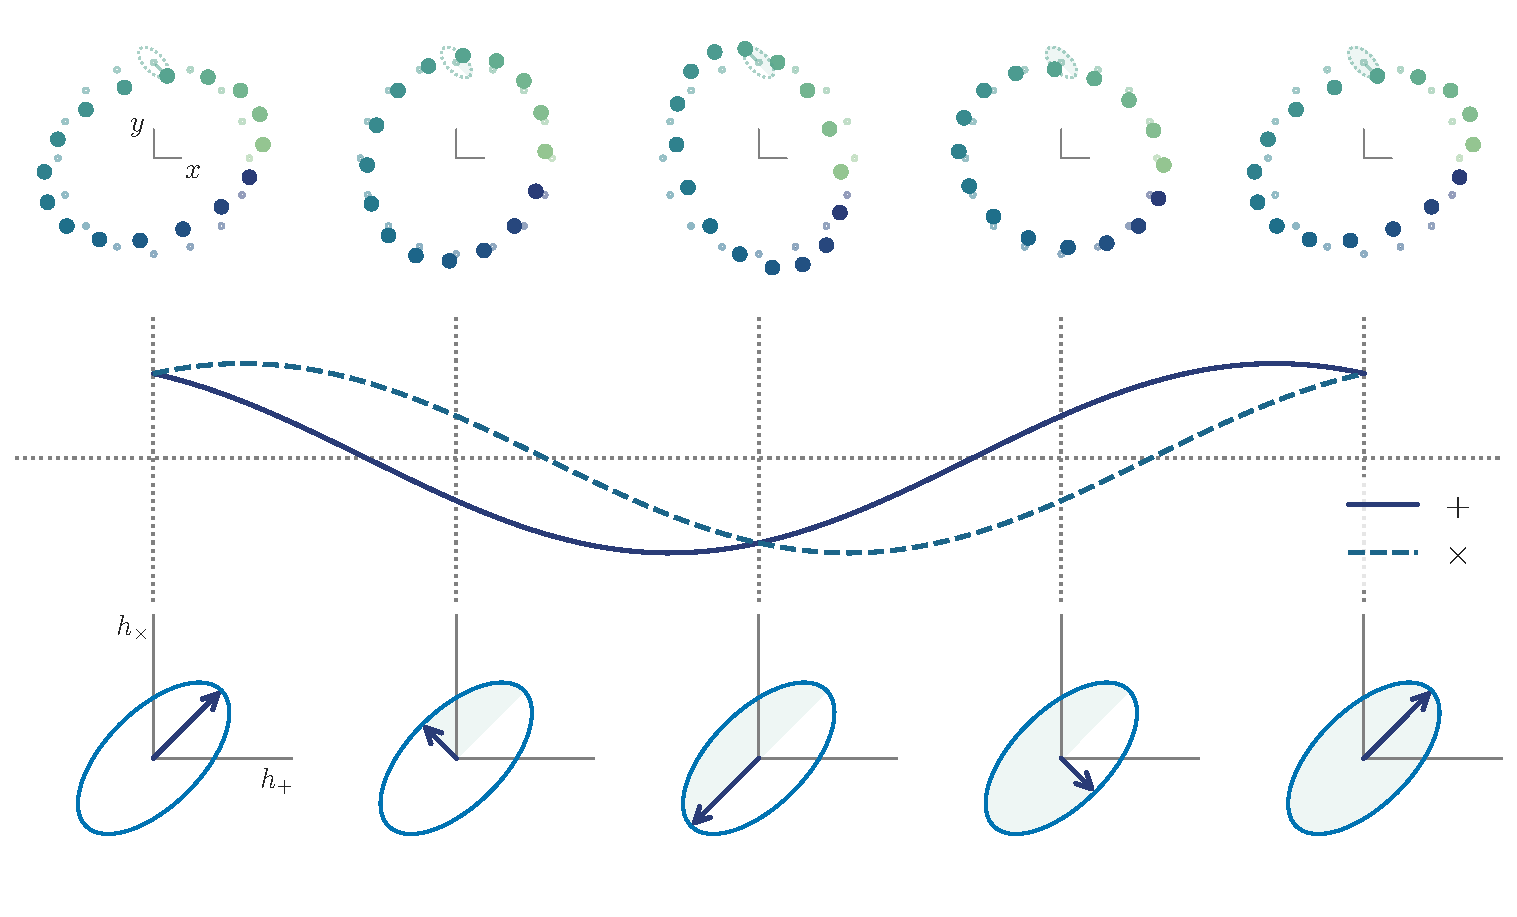
\includegraphics[width=0.8\textwidth]{pol_diagram_ellip}
%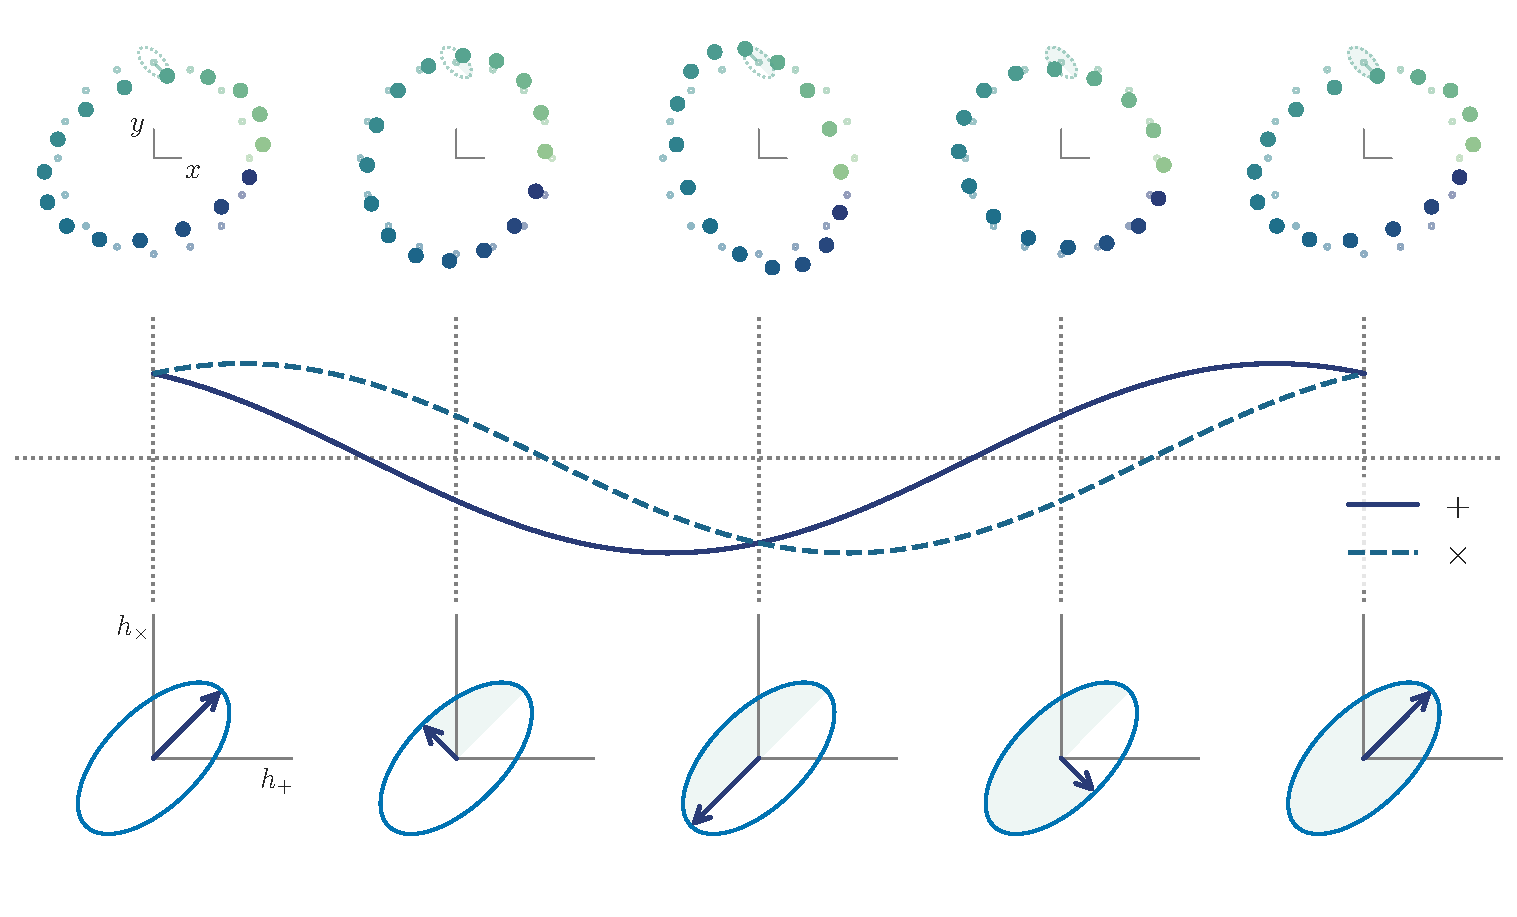
\includegraphics[width=\columnwidth]{pol_diagram_ellip}
\caption{An elliptically polarized GW as a function of time (left to right) over a period, described by Eq.~\eqref{eq:hcomp_ellip} with $\epsilon=1/2$, $\theta=\pi/2$, $\phi=0$ and arbitrary amplitude. \emph{Top:} as the wave propagates out of the page, it deforms a freely falling ring of particles (colored dots) into an ellipsoidal pattern, which in this case rotates counterclockwise with time, albeit nonrigidly; each individual particle is pushed in an ellipse with the same ellipticity as the wave itself, and oriented at an angle $\theta + \varphi$ from the $x$-axis, where $\varphi$ is the polar coordinate locating the particle around the ring.
\emph{Middle:} amplitudes of the plus (solid) and cross (dashed) linear polarizations making up the wave as a function of time.
\emph{Bottom:} representation of the polarization state as a Jones vector in the $+$ and $\times$ space; the phasor rotates counterclockwise as in Fig.~\ref{fig:ellipse}.
}
\label{fig:pol_diagram_ellip}
\end{figure*}

The mathematical treatment of polarized GW states is entirely analogous to the electromagnetic case.
To start, any of these states can be represented graphically by series of phasor diagrams like the one in Fig.~\ref{fig:ellipse}, as in the bottom of Figs.~\ref{fig:pol_diagram_circ} and \ref{fig:pol_diagram_ellip}.
For monochromatic modes (i.e., of a definite $\omega$), the same information can also be encoded algebraically in a complex valued \emph{Jones vector} $\vec{C}$ like 
% Any fully-polarized state can be represented by phasor diagrams like the one in Fig.~\ref{fig:ellipse}.
% Additionally, for a monochromatic mode, the time dependence of the phasor can be factored out so that the whole state is encoded in a \emph{Jones vector} $\vec{A}$ like
\beq \label{eq:jones}
\begin{pmatrix}
h_+\\
h_\times
\end{pmatrix} \equiv
\Re \left[ \begin{pmatrix}
C_+\\
C_\times
\end{pmatrix} e^{-i\omega t}\right] \equiv
\Re \left[ \vec{C}\, e^{-i\omega t}\right] .
\eeq
%just as is standard for electromagnetic waves.
For example, in that notation, $\vec{C}=\left(1, 0\right)$ encodes a unit-amplitude linearly polarized $+$ mode, while $\vec{C} = \left(1,i\right)/\sqrt{2}$ encodes a circular R mode.
We will briefly make use of Jones vectors to facilitate coordinate transformations below.

We can obtain another useful parametrization for fully polarized states by replacing the ellipticity parameter $\epsilon$ in \eq{hcomp_ellip} with an angle $\chi \equiv \arctan \epsilon$, which is also illustrated in Fig.~\ref{fig:ellipse}.
In terms of this quantity and the intensity amplitude $\hat{A}=A\sqrt{1+\epsilon^2}=A \sec\chi$, the elliptical mode of \eq{hcomp_ellip} becomes
\begin{subequations} \label{eq:hcomp_ellip_chi}
\beq
h_+ = \hat{A} \left[\cos\chi \cos \theta \cos(\omega t - \phi) - \sin\chi \sin \theta \sin(\omega t - \phi)\right] ,
\eeq
\beq
h_\times = \hat{A} \left[\cos\chi \sin \theta \cos(\omega t - \phi) + \sin\chi \cos \theta \sin(\omega t - \phi)\right] ,
\eeq
\end{subequations}
Now, $\chi = 0$ gives a linearly polarized state, while $\chi=\pm \pi/4$ gives a R/L circularly polarized state.
Its domain is given by $-\pi/4 \leq \chi \leq \pi/4$, as implied by $-1 \leq \epsilon \leq 1$, and we can further limit $0 \leq \theta \leq \pi$, since \eq{hcomp_ellip_chi} is invariant under $\{\theta \to \theta + \pi, \chi \to \chi + \pi\}$.
% Additionally, the transformation $\{\theta \to \theta \pm \pi/2, \chi \to \pi/2 - \chi, \phi \to \phi \pm \pi/2\}$, with matching signs for the two $\pm \pi/2$ terms, leaves the equation unchanged; this means we can tighten the ranges to $0 < \theta < \pi/2$.

We now have two angles that fully define the shape of the polarization ellipse, $\chi$ and $\theta$.
If we interpret $-\pi/2 \leq 2\chi \leq \pi/2$ and $0 \leq 2\theta \leq 2\pi$ respectively as latitude and longitude coordinates, then the space of all unique polarization states can be arranged into a sphere such that linear polarization states of different orientations live on the equator ($\chi = 0$), and circular states live on the poles ($2\chi = \pm \pi/2$) \cite{poincare,goldstein}.
Any two antipodal states in this so-called \emph{Poincar\'e sphere} can function as a polarization basis.
In this language, reexpressing Eq.~\eqref{eq:planewave} as Eq.~\eqref{eq:planewave_circ} amounted to effecting a Poincar\'{e} rotation of our basis vectors.
The polarization ellipse (Fig.~\ref{fig:ellipse}) can be recovered from the Poncar\'e sphere by a stereographic projection.

If we scale the radius of the Poincar\'{e} sphere to be the signal intensity $I \equiv \hat{A}^2$, then it can be defined in terms of Cartesian coordinates corresponding to the three other \emph{Stokes parameters} that characterize the distribution of power in the signal accross different polarization states \cite{Anile1974}.
For a fully polarized monochromatic mode, in addition to $I$ itself, these are given by
\begin{subequations} \label{eq:stokes}
\beq
Q \equiv |C_+|^2 - |C_\times|^2 = \hat{A}^2 \cos 2\chi \cos 2\theta \, , 
\eeq
\beq
U \equiv C_+ C_\times^* + C_+^* C_\times = \hat{A}^2 \sin2\chi \sin 2\theta \,  ,
\eeq
\beq
V \equiv |C_R|^2 - |C_L|^2 = \hat{A}^2 \sin 2\chi \, ,
\eeq 
\end{subequations}
for $C_+ = (C_R + C_L)/\sqrt{2}$ and $C_\times = i (C_R - C_L)/\sqrt{2}$.
As implied by the definitions above, $Q/I$ controls the (power) fraction of linear polarization, $U/I$ the orientation of the linear component, and $V/I$ the fraction of circular polarization.
The Poincar\'{e} sphere is then the sphere of radius $I$ centered on $\left(Q=0, U=0, V=0\right)$.

For a fully polarized state, the Stokes parameters (quantifying signal power) are equivalent to the polarization quantitites $\left\{A, \epsilon, \theta\right\}$ or $\{\hat{A}, \chi, \theta\}$ defining the ellipse in Fig.~\ref{fig:ellipse} (and quantifying signal amplitude).
Because they are defined in terms of power, Stokes parameters have the advantage of being easily generalizable to fully or partially unpolarized waves, which can be achieved by replacing the definition in Eq.~\eqref{eq:stokes} with corresponding two-point correlation functions (power spectra); in the fully-unpolarized case, $Q=U=V=0$ and there is no Poincar\'{e} sphere to speak of.
The Stokes parameters are thus especially useful when dealing with stochastic signals \cite{Romano:2016dpx,Conneely:2018wis,Seto:2008sr,Kato:2015bye}; since we will be dealing mainly with coherent signals, we will not make further reference to Stokes parameters in what follows.

% Consequently, its applicability extends beyond the formal Fourier expansion in \eq{hcomp_fd_rl} to any context in which the signal (or a component thereof) can be described as having a definite polarization state (which may potentially evolve adiabatically).

\subsection{Non-monochromatic modes}

% \subsubsection{Fully-polarized non-monochromatic states}

We arrived at the expression for a fully-polarized, monochromatic GW in Eq.~\eqref{eq:hcomp_ellip} by way of the generic Fourier decomposition of a plane wave in Eq.~\eqref{eq:hcomp_fd_rl}, wherein elliptical modes appear naturally with a determinate frequency.
Yet, we may also speak of fully-polarized states even if the signal is not monochromatic.

The argument applies to any high-frequency coherent wave, i.e., any wave that can be written as a slow-varying amplitude modulating a fast phase.
In that case, the polarization parameters $\{A, \epsilon, \theta\}$ can be defined instantaneously using the stationary phase approximation or similar procedures.
This way, any GW with a constant polarization state, i.e., whose polarization ellipse takes a fixed, determinate shape (but not necessarily scale), can be encapsulated by an expression of the form
\begin{subequations} \label{eq:ellip_gen}
\begin{equation} %\label{eq:ellip_sum_p}
h_+ = \mathcal{A}(t) \left[\cos \Phi(t) \cos \theta - \epsilon \sin \Phi(t) \sin\theta \right] ,
\end{equation}
\begin{equation} %\label{eq:ellip_sum_c}
h_\times = \mathcal{A}(t) \left[ \cos \Phi(t) \sin \theta + \epsilon \sin \Phi(t) \cos\theta \right] ,
\end{equation}
\end{subequations}
enhancing Eq.~\eqref{eq:hcomp_ellip} with a (slowly) time varying amplitude $\mathcal{A}(t)$ and a (quickly) time varying phase $\Phi(t)$, which need no longer grow linearly with time.
Following this expression, the aspect ratio and orientation of the polarization ellipse remains constant,%
\footnote{The shape of the ellipse could also be made to vary adiabatically via $\epsilon$ and $\theta$ but that is seldomly done in real-world applications.}
while its size may increase or decrease according to $\mathcal{A}(t)$.
The initial state of the signal is defined by the initial amplitude $A = \mathcal{A}(t=0)$ and phase $\phi = \Phi(t=0)$.

Most signals conceivable signals are neither monochromatic nor fully polarized.
Nevertheless, a large variety of morphologies can be captured with a finite superposition of elliptically polarized modes, potentially with time-varying polarization parameters as above.
This should be apparent from the fact that an (uncountably) \emph{infinite} set of elliptical modes can describe \emph{any} GW signal, as we showed in \eq{hcomp_fd_rl}.
For many practical applications, it is advantageous to decompose signals into 
sums of fully-polarized modes in the shape of \eq{ellip_gen},
% \begin{subequations}
% \begin{align}
% h_+ = \sum_n A_n(t) &\left[\cos \theta_n \cos(\omega_n t - \phi_n) \right. \\
% &\left. - \epsilon_n \sin \theta_n \sin(\omega_n t - \phi_n)\right] ,\nonumber
% \end{align}
% \begin{align}
% h_\times = \sum_n A_n(t) &\left[\sin \theta_n \cos(\omega t - \phi_n) \right. \\
% &\left.+ \epsilon \cos \theta \sin(\omega t - \phi_n)\right] , \nonumber
% \end{align}
% \end{subequations}
\begin{subequations} \label{eq:ellip_sum}
\begin{equation} \label{eq:ellip_sum_p}
h_+ = \sum \hspace{-1pt} \mathcal{A}_i(t) \hspace{-1pt} \left[\cos \Phi_i(t) \cos \theta_i - \epsilon_i \sin \Phi_i(t) \sin\theta_i \right] ,
\end{equation}
\begin{equation} \label{eq:ellip_sum_c}
h_\times = \sum \hspace{-1pt} \mathcal{A}_i(t) \hspace{-1pt} \left[ \cos \Phi_i(t) \sin \theta_i + \epsilon_i \sin \Phi_i(t) \cos\theta_i \right] ,
\end{equation}
\end{subequations}
with a sum over some number of modes indexed by $i$, with amplitudes and phases taking some prescribed functional form for each $i$.

The form of Eq.~\eqref{eq:ellip_sum} is flexible enough that it can be used in practice to model arbitrary signals in real detector data.
For example, that is the strategy taken by \textsc{BayesWave} \cite{Cornish:2014kda,Cornish:2020dwh}, which reconstructs generic GW signals by fitting a variable number of elliptically-polarized sine-Gaussians.%
\footnote{\textsc{BayesWave} can currently operate in two configurations: one which assumes the overall signal is elliptically polarized, and another which does not.}
It is also the case, in ringdown studies that fit the final portion of a compact binary signal as a superposition of elliptically polarized damped sinusoids \cite{Isi:2021iql}.

For such applications, each phasing function will usually correspond to some given frequency $\omega_i$ as in a Fourier expansion, so that $\Phi_i(t) = \omega_i t + \phi_i$; meanwhile, the $\mathcal{A}_i(t)$ functions encode amplitude envelopes evolving slowly over some timescale $\tau_i \equiv 1/\gamma_i$.
For example, in the case of ringdown templates, $\mathcal{A}_i(t) = A_i \exp(-\gamma_i t)$ and $\Phi_i(t) = \omega_i t + \phi_i$, for some set of complex-valued frequencies $\tilde{\omega}_i = \omega_i - i\gamma_i$ to be inferred from the data together with polarization parameters $\{ A_i, \epsilon_i, \theta_i, \phi_i\}$.
Equations \eqref{eq:ellip_sum} can be equivalently written in the frequency domain, as done for the sine-Gaussian basis in \cite{Cornish:2014kda,Cornish:2020dwh}.

The elliptical decomposition of Eq.~\eqref{eq:ellip_sum} allows us to flexibly model a GW signal without assuming full independence of the two GW polarizations.
This is justified because, as argued in \cite{Chatziioannou:2021mij}, we expect both polarizations to be generated by the same physical processes, so that their spectral properties should not be totally independent.
Moreover, even if there was a choice of waveframe in which the two linear polarizations looked completely dissimilar, the polarizations will look spectrally similar to generic observers whose frame is randomly oriented.

Besides the modeling of generic signals, \eq{ellip_sum} serves as the exact representation of several classes of astrophysically-relevant signals.
The most salient example of this, as we will see below, is that of compact binary coalescences (CBCs); in particular, a nonprecessing, quasicircular CBC dominated by the quadrupolar angular harmonic of the radiation can be described by a single, fully polarized component, as in \eq{ellip_gen}.

% In fact, as we will see below, the simplest of those signals (viz., nonprecessing inspiral dominated by the quadrupolar angular harmonic) can be described by a single mode like the summand of \eq{hcomp_ellip}, with fixed ellipticity and polarization angle.


\subsection{Relation to spherical harmonics}
\label{sec:harmonics}

When modeling specific sources (e.g., in a numerical-relativity simulation), it is common to decompose the outgoing strain in terms of spin-weighted spherical harmonics ${}_{-2} Y_{\ell m}$ in the frame of the source (e.g., \cite{Kidder:2007rt}), so that, for a detector infinitely far away, we can write
% \begin{align}
% h_+ - i h_\times = \sum_\ell \sum_{m>0} &\left[ H_{\ell m}(t)\, {}_{-2}Y_{\ell m} (\iota, \varphi) + \right. \nonumber \\
% &\left. H_{\ell-m}(t)\, {}_{-2}Y_{\ell -m} (\iota, \varphi) \right]
% \end{align}
\begin{align} \label{eq:spherical}
h_+ - i h_\times = \sum_{\ell \geq 2} \sum_{-\ell \leq m \leq \ell} H_{\ell m}(t)\, {}_{-2}Y_{\ell m} (\iota, \varphi)\, ,
\end{align}
for a source seen with inclination $\iota$ and azimuthal angle $\varphi$, with intrinsic time-dependence encoded in the $H_{\ell m}$ functions as determined by Einstein's equations.
The decomposition into spherical harmonics presumes the choice of both (1) a polar frame defining $\iota$ and $\varphi$, and (2) an orientation of the waveframe vectors with respect to the direction of propagation to establish the meaning of $h_{+/\times}$ as in \eq{hij}.
In the LIGO convention (which follows \cite{Blanchet:2008je,Faye:2012we}), the waveframe in \eq{spherical} is defined by $\hat{x} = - \hat{e}_\varphi$ and $\hat{y} = \hat{e}_\iota$ \cite{LALSuite:source}, and the overall polar frame is centered on and comoving with the source, with an orientation following its symmetries (e.g., aligned with the orbital plane).

The different $H_{\ell m}$'s in \eq{spherical} are generated by the time evolution of specific current and mass moments of the source \cite{Thorne:1980ru}.
As such, their structure must reflect the symmetries of Einstein's equations, including parity.
In particular, for any source satisfying equatorial-reflection (planar) symmetry, like a nonprecessing inspiral, parity can be shown to imply that $H_{\ell -m} = (-1)^\ell H_{\ell m}^*$ \cite{Faye:2012we}.
Allowing for a generic (slow) amplitude and (fast) phase evolution by writing $H_{\ell m}(t) = \mathcal{A}_{\ell m}(t) \exp[-i \Phi_{\ell m}(t)]$, this symmetry reduces to $\mathcal{A}_{\ell -m}(t) = (-1)^\ell \mathcal{A}_{\ell m}(t)$ and $\Phi_{\ell m}(t) = - \Phi_{\ell -m}(t)$, where we have taken $\mathcal{A}$ and $\Phi$ to be real valued.
In that case, \eq{spherical} can be rewritten with an explicit term for negative values of $m$ as
\begin{widetext}
\begin{subequations} \label{eq:spherical_modes}
\begin{align}
h_+ - i h_\times &= \sum_{\ell \geq 2} \sum_{0\leq m \leq \ell} \left[H_{\ell m}(t)\, {}_{-2}Y_{\ell m} (\iota, \varphi) + H_{\ell -m}(t)\, {}_{-2}Y_{\ell -m} (\iota, \varphi) \right] \\
&= \sum_{\ell \geq 2} \sum_{0\leq m \leq \ell} \left[\mathcal{A}_{\ell m}(t)\, e^{-i\Phi_{\ell m} (t)} {}_{-2}Y_{\ell m}(\iota, \varphi) +  (-1)^\ell \mathcal{A}_{\ell m}(t)\, e^{i\Phi_{\ell m} (t)} {}_{-2}Y_{\ell- m}(\iota, \varphi) \right] \\
&= \sum_{\ell \geq 2} \sum_{0\leq m \leq \ell} \left[C_{\ell m} e^{-i\Phi_{\ell m} (t)}  +  C_{\ell -m} e^{i\Phi_{\ell m} (t)} \right]\, ,
\end{align}
\end{subequations}
\end{widetext}

% The different $H_{\ell m}$'s in \eq{spherical} are generated by the time evolution of specific current and mass moments of the source, and, therefore, are often associated with specific signal frequencies \cite{Thorne:1980ru}.
For example, the dominant $\ell= |m|=2$ mode in a nonprecessing compact binary inspiral will evolve with a signal freqyency $\omega_{22}$ which is twice the orbital frequency $\omega_\mathrm{orb}$ or, more generally for other harmonics, $\omega_{\ell m} = m\, \omega_\mathrm{orb}$, with parity invariance requiring $\omega_{\ell m}= - \omega_{\ell - m}$.
If that harmonic structure holds, then Eq.~\eqref{eq:spherical} is equivalent to the elliptical decomposition of Eq.~\eqref{eq:ellip_sum}, as we proceed to show.

For concreteness, represent the $H_{\ell m}$ schematically as simple monochromatic components $H_{\ell m} (t) = \mathcal{C}_{\ell m} \exp\left(-i \omega_{\ell m} t\right)$, where $\mathcal{C}_{\ell m}$ is some complex-valued amplitude, that could be varying slowly with time (slower than $\omega_{\ell m}$).
We can then refactor Eq.~\eqref{eq:spherical} so that we only sum over nonnegative values of $m$,
% \begin{widetext}
% \begin{subequations} \label{eq:spherical_modes}
% \begin{align}
% h_+ - i h_\times &= \sum_{\ell \geq 2} \sum_{0\leq m \leq \ell} \left[H_{\ell m}(t)\, {}_{-2}Y_{\ell m} (\iota, \varphi) + H_{\ell -m}(t)\, {}_{-2}Y_{\ell -m} (\iota, \varphi) \right] \\
% &= \sum_{\ell \geq 2} \sum_{0\leq m \leq \ell} \left[\mathcal{C}_{\ell m} e^{-i\omega_{\ell m} t} {}_{-2}Y_{\ell m}(\iota, \varphi) +  \mathcal{C}_{\ell -m} e^{i\omega_{\ell m} t} {}_{-2}Y_{\ell- m}(\iota, \varphi) \right] \\
% &= \sum_{\ell \geq 2} \sum_{0\leq m \leq \ell} \left[C_{\ell m} e^{-i\omega_{\ell m} t}  +  C_{\ell -m} e^{i\omega_{\ell m} t} \right]\, ,
% \end{align}
% \end{subequations}
% \end{widetext}
where, in the last line, we have absorbed the angular factors into $C_{\ell m} \equiv {}_{-2}Y_{\ell m} (\iota, \varphi)\, \mathcal{C}_{\ell m}$.

The summand in the last line of \eq{spherical_modes} takes the form of \eq{ellip_circ}, and its interpretation is the same: each $(\ell$, $|m|)$ contributes a single, elliptically polarized mode to the waveform.
The amplitude and ellipticity of each mode are determined by both (1) the intrinsic amplitudes $\mathcal{C}_{\ell \pm m}$, and (2) the viewing angle $(\iota, \varphi)$, through the ${}_{-2} Y_{\ell m}$ factors.
Although we have simplified \eq{spherical_modes} by taking each $(\ell, m)$ mode to be monochromatic, we would have arrived at the same conclusion regarding polarizations had we instead allowed for a generic (slow) amplitude and (fast) phase evolution by writing $H_{\ell m}(t) = \mathcal{A}_{\ell m}(t) \exp[-i \Phi_{\ell m}(t)]$, for real valued $\mathcal{A}_{\ell m}$ and with parity invariance now requiring $\Phi_{\ell m}(t) = - \Phi_{\ell -m}^*(t)$; in that case the last line of \eq{spherical_modes} would have taken the form of \eq{ellip_sum}, with each summand representing a fully polarized, albeit non-monochromatic, mode.

A special case of Eq.~\eqref{eq:spherical_modes} is that of a nonprecesing compact binary inspiral.
In that case, equatorial-reflection (planar) symmetry implies that $H_{\ell -m} = (-1)^\ell H_{\ell m}^*$ \cite{Faye:2012we}.
The strain for a given $(\ell, |m|)$ mode can then be written as
\begin{equation}
h_+ - i h_\times = \mathcal{A}_{\ell m} \left[ Y^+_{\ell m} \cos \Phi_{\ell m}(t) - 
i Y^\times_{\ell m} \sin \Phi_{\ell m}(t) \right]\hspace{-3pt} ,
\end{equation}
where we have used $H_{\ell m}(t) = \mathcal{A}_{\ell m}(t) \exp[-i \Phi_{\ell m}(t)]$ and defined
\begin{equation}
Y_{\ell m}^{+/\times}(\iota,\varphi) \equiv {}_{-2} Y_{\ell m}(\iota, \varphi) \pm {}_{-2} Y_{\ell m}(\pi-\iota, \varphi + \pi) \, ,
\end{equation}
with the plus (minus) sign for the plus (cross) polarization (see Appendix B of \cite{Isi:2021iql}); here we have used the symmetry that ${}_{-2} Y_{\ell -m}(\iota,\varphi) = (-1)^{\ell+m} {}_{-2} Y_{\ell m}^*(\pi-\iota,\varphi+\phi)$ \cite{goldberg:1967}.
This implies that that, for a nonprecessing binary, the ellipticity of each $(\ell, |m|)$ mode is determined only by the source inclination.
For the special case of the dominant $\ell=|m|=2$ mode, this reduces to the familiar expression in terms of $\cos\iota$,
\begin{subequations}
\beq
h_+ = \frac{1}{2} \sqrt{\frac{5}{4\pi}} \mathcal{A}_{22} \left(1 + \cos^2\iota\right) \cos \Phi_{22}(t) \, , 
\eeq
\beq
h_\times = \sqrt{\frac{5}{4\pi}} A'_{22}  \cos\iota \sin \Phi_{22}(t) \, .
\eeq
\end{subequations}
The ellipticity for such a signal is thus a pure function of the inclination, namely
\beq \label{eq:ellip_cosi}
\epsilon = \frac{2 \cos\iota}{1+\cos^2\iota}\, . 
\eeq


\section{Polarization angles}

\subsection{Wave-frame and the angle $\psi$}
\label{sec:pol}

Equation \eqref{eq:hij} presumes a specific choice of frame orientation that defines the basis in which the $h_{ij}$ components are written.
Although \eq{hij} requires that $\hat{z}$ be parallel to the (spatial) wave vector $\vec{k}$, there is no a priori restriction on the orientation of the $x$ and $y$ axes within the plane perpendicular to $\vec{k}$.
This freedom is usually encapsulated in the choice of an arbitrary \emph{polarization angle} $\psi$, defined with respect to some convenient absolute reference.
For instance, in the LIGO convention, this angle is defined with respect to celestial coordinates such that $\psi=0$ means that the waveframe $\hat{x}$ is parallel to the celestial equator \cite{LALSuite:wave}.

With some trigonometry, it is straightforward to show that a rotation by some angle $\Delta \psi$ around $z$ leaves the form of \eq{hij} unchanged after redefining
\beq \label{eq:htransf}
h_+ \rightarrow h_+' = h_+ \cos 2\Delta \psi - h_\times \sin 2\Delta\psi \, ,
\eeq
\beq
h_\times \rightarrow h_\times' = h_\times \cos 2\Delta \psi + h_+ \sin 2\Delta\psi \, .
\eeq
This reveals the fact that $h_+$ and $h_\times$ are nothing but the two components of a tensor field with spin-weight $|s|=2$, and the two polarizations are only defined up to an arbitrary choice of $\psi$.

Under rotations of the wave frame, the antenna patterns of \eq{h} transform through an expression complementary to \eq{htransf},
\begin{subequations} \label{eq:Ftransf}
\beq
F_+ \rightarrow F_+' = F_+ \cos 2\Delta \psi + F_\times \sin 2\Delta\psi \, ,
\eeq
\beq
F_\times \rightarrow F_\times' = F_\times \cos 2\Delta \psi - F_+ \sin 2\Delta\psi \, ,
\eeq
\end{subequations}
ensuring that the observable $h(t)$ in \eq{h} is independent of the arbitrary angle $\psi$.
More generally, any scalar like $D^{ij} e^{p}_{ij}$ will necessarily be frame invariant.%
\footnote{This extends to gauge transformations: the spacetime tensors $D_{ab}$ and $h_{ab}$ are gauge dependent, but their innerproduct is not.}

Unlike the linear modes of Eq.~\eqref{eq:lin}, the tensors of Eq.~\eqref{eq:circ} do not mix under rotations around the direction of propagation:
the circular polarizations are eigenstates of the helicity operator with weight $\pm 2$, corresponding to the two helicities of a spin-2 massless particle (see, e.g., \cite{Hinterbichler2011}).
The equivalent transformation to Eq.~\eqref{eq:htransf} is
\begin{subequations} \label{eq:htransf_circ}
\begin{align}
h_R &\rightarrow h_R' = h_R \exp(- i2  \Delta \psi) \, ,\\
h_L &\rightarrow h_L' = h_L \exp(+ i2  \Delta \psi)\, ,
\end{align}
\end{subequations}
meaning that a rotation around $\hat{z}$ is equivalent to a simple change in the overall phase of the circular polarization components.
As such, a change in $\psi$ can be absorbed by a redefinition of the Fourier phases in \eq{hcomp_fd_rl}, multiplying the integral through by $\exp(-i2\Delta\psi)$.

The definition of the angle $\psi$ (with respect to, say, the celestial equator) is not intrinsically related to any feature of the signal: it simply defines an arbitrary frame in which to prescribe the $h_+$ and $h_\times$ polarization functions in \eq{hij}, or equivalently, the frame in which to measure the phases of the circularly polarized Fourier components.
Nevertheless, even though any choice of $\psi$ is formally valid, specific signal morphologies may make some choices more convenient than others.


\subsection{Elliptical waves and the angle $\theta$}
\label{sec:ellip}

Another notion of ``polarization angle'' arises naturally in the description of elliptically polarized signals.
The expression for an elliptical wave in \eq{ellip_gen} presumes some specific choice of $\psi$ that defines the meaning of plus vs cross by orienting $\hat{x}$, as explained in the previous section.
The expression simplifies if we choose that angle such that the plus and cross axes are aligned with the principal components of the ellipse, i.e., constructing the polarization frame to ensure that $\theta = 0$ (see Fig.~\ref{fig:ellipse}).

With such a choice of wave frame (equivalently, choice of $\psi$), \eq{ellip_gen} becomes just
\begin{subequations} \label{eq:ellip_frame}
\beq
h_+ = \mathcal{A}(t) \cos \Phi(t) \, ,
\eeq
\beq
h_\times = \epsilon \mathcal{A}(t) \sin \Phi(t)\, .
\eeq
\end{subequations}
Crucially, an elliptical wave will generally not take the form of Eq.~\eqref{eq:ellip_frame} unless $\hat{x}$ is chosen appropriately; only circularly polarized signals ($\epsilon=\pm1$) will take  this simplified form irrespective of the wave frame orientation (again showing that these are eigenstates of the helicity operator).

Therefore, when working with a single elliptically-polarized wave, Eq.~\eqref{eq:ellip_frame} defines a privileged orientation of the wave frame, unique up to rotations by $\pi/2$ around $\hat{z}$.
If we adopt $\theta =0$ as a convention (or, equivalently, $\theta=\pi$), then we \emph{define} our wave frame to lie along the principal axes of the polarization ellipse and, thus, the polarization angle $\psi$ becomes synonymous with the polarization ellipse orientation.
However, the two angles $\theta$ and $\psi$ are conceptually distinct; in particular, $\theta$ is defined only for elliptically polarized waves, whereas $\psi$ is always defined.

% where the source sky location is parametrized by its right ascension $\alpha$ and declination $\delta$.

As for any GW, the detector output for an elliptically polarized wave will be given by \eq{h}.
In this case, however, \eq{Ftransf} implies that $\psi$ and $\theta$ are degenerate, as detailed in Appendix A of \cite{Isi:2017equ}.
Concretely, for a fixed sky location (i.e., propagation direction), a change from $\psi \to \psi' = \psi + \Delta\psi$ in the antenna patterns can be absorbed by a change in $\theta$ because the expression
\beq
h = F_+(\psi + \Delta \psi) h_+ + F_\times(\psi + \Delta \psi) h_\times 
\eeq
can be expanded by means of \eq{Ftransf} to read
\begin{align}
h = &\left[ F_+(\psi) \cos 2\Delta\psi + F_\times(\psi) \sin 2\Delta\psi \right] h_+\, + \\
 &\left[F_\times(\psi) \cos 2\Delta\psi - F_+(\psi)\sin 2\Delta\psi\right] h_\times \, .
\end{align}
Plugging in the expressions for an elliptical wave in \eq{ellip_gen} and taking advantage of trigonometric identities, this can be rearranged into
\begin{widetext}
\begin{align} \label{eq:theta_psi}
h = & \mathcal{A}(t) \left[\cos \Phi(t) \cos(\theta + 2\Delta\psi) -  \epsilon \sin \Phi(t)\sin(\theta + 2\Delta\psi) \right] F_+(\psi) +\nonumber\\
&\mathcal{A}(t) \left[\cos \Phi(t) \sin(\theta + 2\Delta\psi) + \epsilon \sin \Phi(t) \cos(\theta + 2\Delta\psi) \right] F_\times(\psi), 
\end{align}
\end{widetext}
which is the same result we would have obtained by replacing $\theta \to \theta' = \theta + 2 \Delta\psi$ in \eq{ellip_gen}.
We could have equivalently (and more quickly) derived this by noting that $\theta$ is related to the phases of the circularly-polarized components of the signal by $\theta = \left(\phi_L - \phi_R\right)/2$, as in \eq{hcomp_ellip}; the transformation rule for $\theta$ then follows from \eq{htransf_circ}, which implies $\phi_{R/L} \to \phi'_{R/L} \mp 2\Delta\psi$, with the negative (positive) sign for R (L).

This implies that elliptical-wave analyses that allow $\theta$ to vary freely should avoid degeneracies by fixing $\psi$ to an arbitrary a priori value.
Choosing this fiducial value to be $\psi=0$, the template at a given detector would be constructed as
\begin{equation}
h = F_+(\psi=0)\, h_+ + F_\times(\psi=0)\,  h_\times \, ,
\end{equation}
for $h_{+/\times}$, as in Eq.~\eqref{eq:ellip_sum}, functions of $\{\theta_i, \epsilon_i\}$ and whatever other parameters are needed to evaluate the amplitude and phasing functions $\{\mathcal{A}_i(t), \Phi_i(t)\}$ (or their frequency-domain analogs).
The antenna patterns $F_{+/\times}$ are evaluated for some sky location and arrival time, which can be allowed to vary to be measured from the data.
On the other hand, the angle $\psi$ is fixed; allowing it to vary would amount to shifting all $\theta_i$ values by $2\psi$, per Eq.~\eqref{eq:theta_psi}.
This was the approach taken in \cite{Isi:2017equ,Chatziioannou:2021mij,Isi:2021iql}.



% \begin{alignat}{2}
% h &= &&\left. F_+(\psi + \Delta \psi) h_+ + F_\times(\psi + \Delta \psi) h_\times\right.  \\
%   &= &&\left[ F_+(\psi) \cos 2\Delta\psi + F_\times(\psi) \sin 2\Delta\psi \right] h_+\, + \\
% & &&\left[F_\times(\psi) \cos 2\Delta\psi - F_+(\psi)\sin 2\Delta\psi\right] h_\times, 
% \end{alignat}
% The (arbitrary) choice to set $\psi=0$ in the antenna pattern evaluation is legitimate because that degree of freedom is fully degenerate with the $\theta_i$ via Eq.~\eqref{eq:Ftransf}, as detailed in Appendix A of \cite{Isi:2017equ}.
% Concretely, a change from $\psi = 0$ to $\psi= \Delta\psi$ can be written as
% \begin{align}
% h = &\left[ F_+(\psi=0) \cos 2\Delta\psi + F_\times(\psi=0) \sin 2\Delta\psi \right] h_+\, +\nonumber\\
% &\left[F_\times(\psi=0) \cos 2\Delta\psi - F_+(\psi=0)\sin 2\Delta\psi\right] h_\times, 
% \end{align}
% suppressing the sky location dependence for simplicity.

% \begin{align}
% h = & \left[h_+ \cos 2\Delta\psi - h_\times \sin 2\Delta\psi \right] F_+(\psi=0) +\nonumber\\
% &\left[h_\times \cos 2\Delta\psi + h_+ \sin 2\Delta\psi\right] F_\times(\psi=0), 
% \end{align}

% \begin{widetext}
% \begin{align}
% h = & \left[A(t) \left[\cos \Phi(t) \cos \theta - \epsilon \sin \Phi(t) \sin\theta \right] \cos 2\Delta\psi - A(t) \left[ \cos \Phi(t) \sin \theta + \epsilon \sin \Phi(t) \cos\theta \right]  \sin 2\Delta\psi \right] F_+(\psi=0) +\nonumber\\
% &\left[A(t) \left[ \cos \Phi(t) \sin \theta + \epsilon \sin \Phi(t) \cos\theta \right]  \cos 2\Delta\psi + A(t) \left[\cos \Phi(t) \cos \theta - \epsilon \sin \Phi(t) \sin\theta \right] \sin 2\Delta\psi\right] F_\times(\psi=0), 
% \end{align}
% \end{widetext}

% \begin{widetext}
% \begin{align}
% h = & A(t) \left[\cos \Phi(t) \left[ \cos 2\Delta\psi\cos \theta - \sin \theta \sin 2\Delta\psi  \right] -  \epsilon  \sin \Phi(t)\left[ \cos 2\Delta\psi \sin\theta+ \cos\theta \sin 2\Delta\psi\right] \right] F_+(\psi=0) +\nonumber\\
% &A(t) \left[\cos \Phi(t) \left[\sin \theta \cos 2\Delta\psi + \cos \theta \sin 2\Delta\psi \right] + \epsilon \sin \Phi(t) \left[\cos\theta \cos 2\Delta\psi - \sin\theta \sin 2\Delta\psi \right] \right] F_\times(\psi=0), 
% \end{align}
% % \end{widetext}
% 
% % \begin{widetext}
% \begin{align}
% h = & A(t) \left[\cos \Phi(t) \cos(\theta + 2\Delta\psi) -  \epsilon \sin \Phi(t)\sin(\theta + 2\Delta\psi) \right] F_+(\psi=0) +\nonumber\\
% &A(t) \left[\cos \Phi(t) \sin(\theta + 2\Delta\psi) + \epsilon \sin \Phi(t) \cos(\theta + 2\Delta\psi) \right] F_\times(\psi=0), 
% \end{align}
% \end{widetext}
% 

\subsection{Compact binaries and the angle $\Psi$}

When modeling GW waveforms from specific systems, it is useful to tie the polarization frame to the geometry of the source.
This is advantageous because, in order to write out explicit expressions for $h_+$ and $h_\times$, we must make \emph{some} definite choice of frame orientation, and doing so in a way that respects the symmetries of the source (if any) can lead to simplified expressions.
That was the case in going from Eq.~\eqref{eq:ellip_gen} to Eq.~\eqref{eq:ellip_frame} above: if we know a priori that the waves from a given source will always be elliptically polarized, then it makes sense to anchor our wave frame to some feature of the source orientation that will ensure alignment with the principal directions of the polarization ellipse (i.e., $\theta=0$).
This is the case for nonprecessing compact binary coalescences (CBCs).
% Furthermore, standardizing the choice reduces ambiguity when reporting $h_{+/\times}$.

For a compact binary, it is conventional to compute the polarizations in a frame such that $\hat{y}$ lies along the intersection of the orbital plane with the plane of the sky (the line of nodes), $\hat{z}$ is parallel to the wave vector as required by \eq{hij}, and $\hat{x}$ completes the triad \cite{LALSuite:source}.
This was the frame assumed in \eq{spherical}.
If the spins of the objects are aligned and the source does not precess, one can show that, in that frame, $h_+$ and $h_\times$ for the dominant ($\ell=|m|=2$) moment of the radiation take the form (e.g., \cite{Poisson2014})
\begin{subequations} \label{eq:cbc}
\beq
h_+ = \left(1 + \cos^2 \iota\right) A(t; R, \vec{\lambda}) \cos \Phi(t; \vec{\lambda}) \, , 
\label{eq:cbc_p} 
\eeq
\beq
h_\times = 2 \cos \iota\, A(t; R, \vec{\lambda}) \sin \Phi(t; \vec{\lambda})\, ,
\label{eq:cbc_c}
\eeq
\end{subequations}
where the inclination $\iota$ is the angle between the orbital angular momentum and the line of sight, and $A(t; \vec{\lambda}) \equiv R  A(t; R, \vec{\lambda})$ and $\Phi(t; \vec{\lambda})$ are some amplitude and phasing functions fully determined by intrinsic source parameters $\vec{\lambda}$.
These quantities include the component masses and spin vectors, a reference phase and, potentially, parameters related to eccentricity and matter effects (like tides).
In the case of an inspiraling compact binary, the $A(t; R, \vec{\lambda})$ and $\Phi(t; \vec{\lambda})$ functions encode a characteristic ``chirping'' signal, but this fact is irrelevant to discussions of polarization structure.
% The inclination $\iota$ is the polar angle with respect to the orbital angular momentum.

\begin{figure}
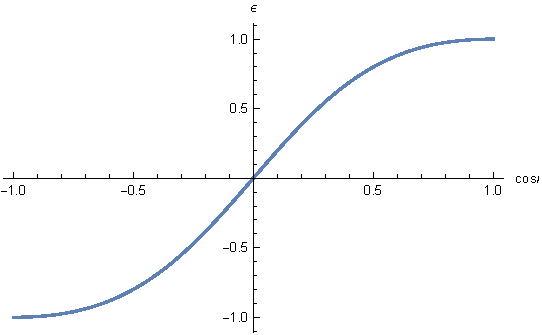
\includegraphics[width=\columnwidth]{ellip_cosi}
\caption{Ellipticity ($\epsilon$, ordinate) as a function of the cosine of the inclination ($\cos\iota$, abscissa) for the $\ell = |m| = 2$ GW strain from a nonprecessing compact binary inspiral, Eq.~\eqref{eq:ellip_cosi}. The signal from a face-on (face-off) binary has ellipticity $\epsilon = +1$ ($\epsilon=-1$), meaning it has a right-handed (left-handed) circular polarization.}
\label{fig:ellip_cosi}
\end{figure}

By comparison with Eq.~\eqref{eq:ellip_frame}, it is clear that Eqs.~\eqref{eq:cbc} describe an elliptically polarized wave in a frame aligned with the polarization ellipse.
This is a consequence of the geometry of our assumed source, which is symmetric under reflections over the orbital plane: by choosing $\hat{y}$ to lie along the line of nodes, we also aligned our wave frame with the GW polarization ellipse.
Since our frame is already aligned  with the ellipse, we may just read off the ellipticity from Eq.~\eqref{eq:cbc}
% \beq \label{eq:ellip_cosi}
% \epsilon = \frac{2 \cos\iota}{1 + \cos^2\iota}\, ,
% \eeq
the ratio of cross to plus amplitudes in this frame, which returns \eq{ellip_cosi} (Fig.~\ref{fig:ellip_cosi}).
%the ratio of cross to plus amplitudes in this frame, and varies between $-1 \leq \epsilon \leq 1$ as required (Fig.~\ref{fig:ellip_cosi}).
This fact reveals that our decision to tie the polarization frame to the line of nodes was a good one: because this choice of wave-frame orientation preserves the symmetries of the source, it also happens to be aligned with the principal directions of the polarization ellipse.

Having specified $h_+$ and $h_\times$ in the standard source-based frame of Eq.~\eqref{eq:ellip_frame}, we need to determine how that frame itself is oriented with respect to the detectors in order to evaluate \eq{h}.
This is most easily done by expressing the components of $h_{ij}$ and $D_{ij}$ in a common basis, usually equatorial celestial coordinates for ground-based detectors.
If we use the standard convention for compact binaries described above (i.e., $\hat{y}$ along the line of nodes), then $\psi = 0$ must mean that the line of nodes points towards the celestial South \cite{LALSuite:source} (equivalently, the projection of orbital angular momentum is parallel to the celestial equator), see  Fig.~\ref{fig:waveframe}.
Knowing this, we can obtain expressions for $h_+$ and $h_\times$ in the celestial frame by measuring the angle from the line of ascending nodes to the celestial south and using \eq{htransf} with $\Delta\psi = \psi - 0 =\psi$.

In this convention, $\psi$ is identical to the \emph{position angle} of the source's orbital angular momentum $\Psi$; more generally, $\Psi = \psi \red{+} \Omega \red{-} \pi/2$ in terms of the longitude of the ascending node $\Omega$ with $\hat{x}$ as the origin of longitude ($\Omega = \pi/2$ in the default LIGO-Virgo convention) \cite{LALSuite:source}.
In fact, for a nonprecessing binary, the three angles $\psi$, $\Psi$ and $\theta$ can all be subsumed by a single parameter (usually written $\psi$) simultaneously encoding the orientation of our polarization basis, the alignment of the source in the sky, and the principal axes of the GW polarization ellipse.
We can then think of this angle as a property of the source to be measured from our data, rather than an arbitrary parameter orienting our frame.
Although this equivocation vastly simplifies analysis, it is useful to keep in mind that the three angles are conceptually distinct.

\begin{figure}
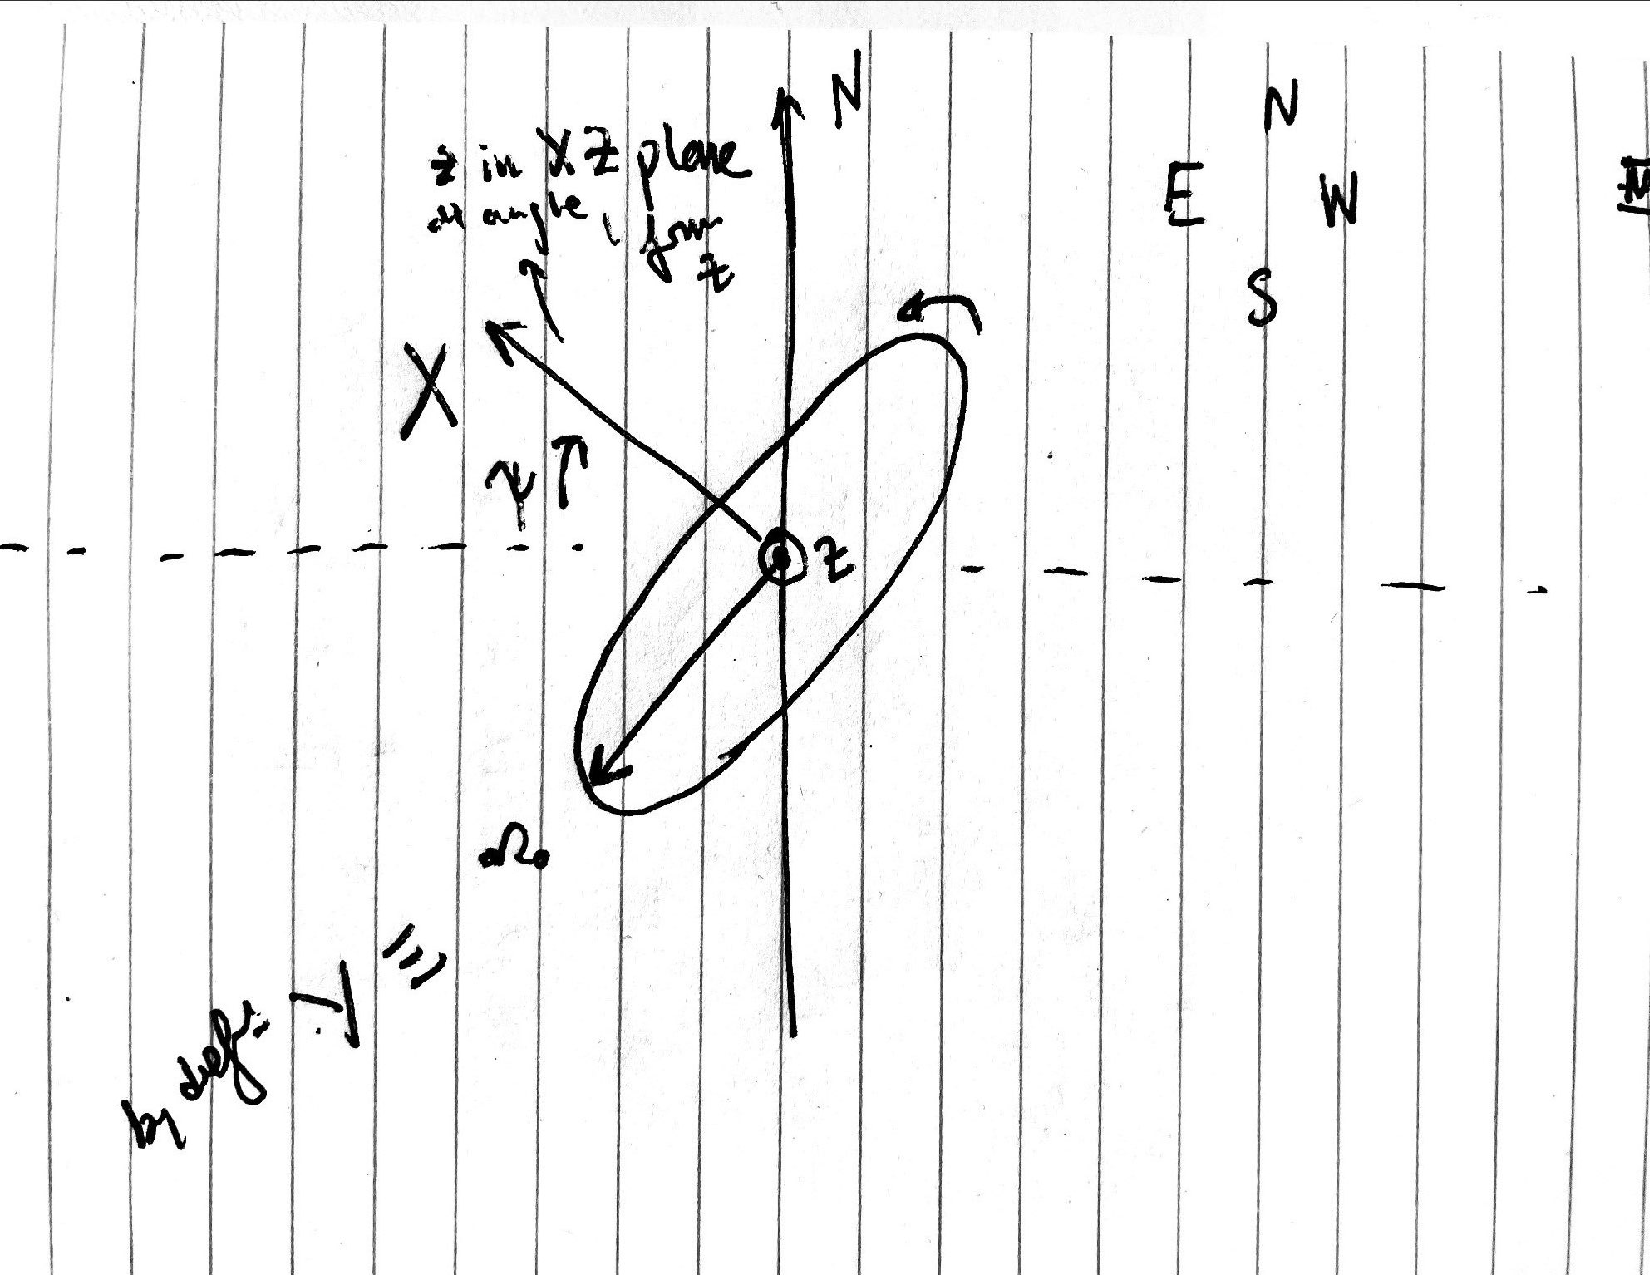
\includegraphics[width=\columnwidth]{waveframe}
\caption{Waveframe for a nonprecessing CBC source.}
\label{fig:waveframe}
\end{figure}

If the component spins are not (anti)aligned with the orbital angular momentum, the spins and the orbital plane will both precess.
As a consequence, the system will not be reflection symmetric and the GW signal will not be elliptically polarized overall.
In that case, it is still conventional to tie $\hat{x}$ to the source, referring to the line of nodes as oriented at some specific point in the binary evolution (e.g., when the detected GW signal reaches 20 Hz).

In summary, we can identify three conceptually distinct Cartesian frames: a wave frame that determines the principal directions along which we \emph{define} the effect of a plus vs cross wave; for an elliptical wave, an intrinsic polarization frame, representing the principal directions of the polarization ellipse; and a source frame, aligned with the symmetries of the source, or otherwise anchored to some defining feature of it; all of these can be specified in some astronomical frame, like ecliptic celestial coordinates.
For nonprecessing binaries, which are highly symmetric, we can define the source frame to make it always align with the polarization frame.

In unomdeled analyses, it is not possible or useful to explicitly tie the polarization frame to properties of the source, since these analyses are not tailored to any specific source to begin with (or they purposely disregard source orientation information).
In that case, the model for $h_+$ and $h_\times$ can be defined in any arbitrary wave frame.
A common choice is to simply set $\psi = 0$ in the standard coordinates described in Sec.~\ref{sec:pol}, i.e., \red{with $\hat{y}$ pointing towards the celestial South} (Fig.~\ref{fig:waveframe}).
Having done so, all information regarding polarization orientation will be encoded in the $\theta$ parameter of Fig.~\ref{fig:ellipse}, with one value per elliptical mode in the decomposition.

\section{Coordinate transformations}

In the previous sections, we have introduced different parametrizations of elliptical (fully polarized) waves, including Eqs.~\eqref{eq:ellip_circ}, \eqref{eq:hcomp_ellip} and \eqref{eq:hcomp_ellip_chi}.
Their use varies depending on the specific application, according to convenience and convention.
Understanding the relation between the different parametrization becomes especially important when implementing and interpreting measurements, since the choice of parametrization affects the prior specified in the analysis.
Measurements obtained with different parametrizations may be related via a Jacobian.

We may also want to switch parametrizations for technical reasons.
Although conceptually insightful, the manifestly-elliptical parameterization in terms of $\{A, \epsilon, \theta, \phi\}$ of \eq{hcomp_ellip} contains multiple degeneracies that make it less than ideal for sampling purposes.
For instance, the angles $\theta$ and $\phi$ become totally degenerate when $\epsilon = \pm 1$; another degeneracy appears as $\theta \to \theta + \pi$ and $\epsilon \to - \epsilon$.
To circumvent this, we may switch to a more suitable parametrization in the sampling process, and then translate the result back into $\{A, \epsilon, \theta, \phi\}$ for interpretation.
In that case, we can still specify a prior in terms of the elliptical quantities by again making use of a Jacobian.

If we parametrize our analysis in terms of some alternative set of parameters $\vec{\xi}$, we can impose some prior distribution $p({A, \epsilon, \theta, \phi})$, defined in the space of elliptical quantities, by choosing a corresponding prior for the $\vec{\xi}$ quantities such that
\begin{equation}
p \left( \vec{\xi} \right) = p \left( A, \epsilon, \theta, \phi \right) \left| \frac{\partial \{A, \epsilon, \theta, \phi\}}{\partial \vec{\xi}} \right| ,
\end{equation}
where the last factor $J \equiv | \partial (A, \epsilon, \theta, \phi)/\partial \vec{\xi} |$ is the determinant of the Jacobian matrix.

In this section, we will consider four different parametrizations of an elliptical wave, and present the Jacobians relating them to the $\{A, \epsilon, \theta, \phi\}$ parametrization.
We will focus on a single elliptical component as a standin for any individual term in the sum of Eq.~\eqref{eq:ellip_sum}, so that the results are trivially generalizable to decompositions of GWs with arbitrary polarizations, as would be used by \textsc{BayesWave} or other generic analyses.
We assume the amplitude could potentially subsume any (slow) time dependence present implied by $\mathcal{A}(t)$ in Eq.~\eqref{eq:ellip_gen}, e.g., the amplitude parameters below could correspond to a reference amplitude $A=\mathcal{A}(t=0)$.

\subsection{Amplitude and ellipticity}

\begin{figure}
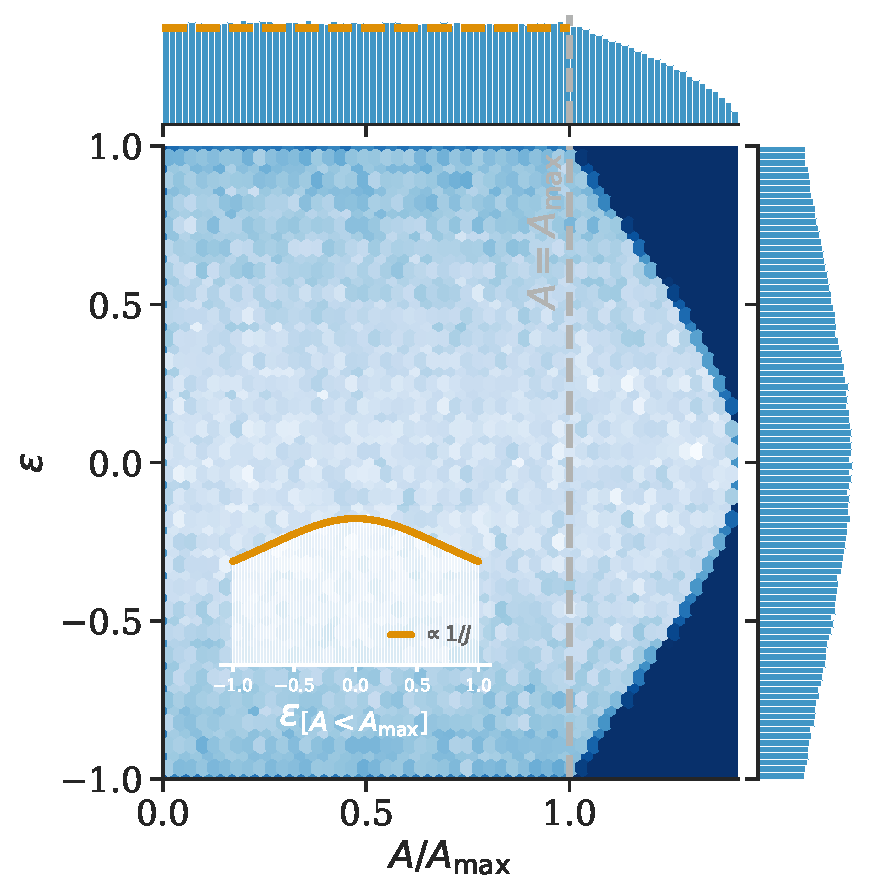
\includegraphics[width=\columnwidth]{jac_Aeps_Achi}
\caption{The Jacobian to be applied in transforming a probability density from $\{\hat{A},\chi\}$ to $\{A,\epsilon\}$, \eq{jac_Aeps_Achi}.
This indicates that a uniform prior on $\hat{A}$ and $\chi$ imposes a distribution that favors linear polarizattions ($\epsilon = 0$) over circular ones ($\epsilon = \pm 1$), with probability density $\propto 1/J_0$. }
\label{fig:jac_Aeps_Achi}
\end{figure}

In Sec.~\ref{sec:ellip:mono}, we presented two equivalent parametrizations of the $h_{+/\times}$ components of an elliptical wave, Eqs.~\eqref{eq:hcomp_ellip} and \eqref{eq:hcomp_ellip}, illustrated in Fig.~\ref{fig:ellipse}.
Equation ~\eqref{eq:ellip_circ} parametrizes the signal strength via the maximum amplitude achieved by the wave, $A$ (the semimajor axis in Fig.~\ref{fig:ellipse}), and the shape of the polarization ellipse via the ellipticity, $\epsilon$ (the ratio between the semiminor and semimajor axes);
meanwhile, Eq.~\eqref{eq:hcomp_ellip_chi} parametrizes the strength via the intensity amplitude $\hat{A}$, which is the square-root of the signal intensity $I$, and the shape of the ellipse throught the angle $\chi$.
The two parametrizations are straigthforwardly related by
\begin{equation} \label{eq:Aellip_Ahatchi}
\begin{cases}
\hat{A} = A \sqrt{1 + \epsilon^2} \\
\chi = \arctan \epsilon 
\end{cases} 
\end{equation}
and the inverse transformation
\begin{equation} \label{eq:Ahatchi_Aellip}
\begin{cases}
A = \hat{A} \cos \chi \\
\epsilon = \tan \chi \\
\end{cases} ,
\end{equation}
with no change to the angles $\theta$ and $\phi$.
The Jacobian relating these two transformations is simply
\begin{equation} \label{eq:jac_Aeps_Achi}
J_0 \equiv \left| \frac{\partial(A,\epsilon,\theta,\phi)}{\partial(\hat{A}, \chi, \theta, \phi)}\right| =  \sec \chi = \sqrt{1 + \epsilon^2}
\end{equation}
or, equivalently $J_0 = \hat{A}/A$.
This Jacobian is illustrated in Fig.~\ref{fig:jac_Aeps_Achi}.



\subsection{Circular components}

An elliptical wave, Eq.~\eqref{eq:hcomp_ellip}, can be specified in terms of the circular polarization basis elements.
If we let,
\begin{align} \label{eq:Cphi}
h_+ - i h_\times = A_{R}\, e^{-i \left(\omega t - \phi_R \right) } + A_{L}\, e^{i \left(\omega t - \phi_L \right) }\, ,
\end{align}
then note that setting $A_L = 0$ ($A_R =0$) results in a fully right-handed (left-handed) circularly polarized wave with amplitude $A_R$ ($A_L$) and phase $\phi_R$ ($\phi_L$).
This form of the strain arose in Eq.~\eqref{eq:ellip_circ}, with $A_{R/L} e^{i\phi_{R/L}} = C_{R/L}/\sqrt{2}$.

The above representation in terms circular-mode amplitudes and phases is equivalent to Eq.~\eqref{eq:hcomp_ellip} if we impose
\begin{equation} \label{eq:Cphi_to_Aellip}
\begin{cases}
A = A_R + A_L \\
\epsilon = (A_R - A_L)/(A_R + A_L) \\ 
\theta = \frac{1}{2}(\phi_L - \phi_R)\\
\phi = \frac{1}{2}(\phi_L + \phi_R)\\
\end{cases} .
\end{equation}
Equivalently, the inverse transformation is 
\begin{equation}
\begin{cases}
A_R = \frac{1}{2} A \left(1 + \epsilon\right) \\
A_L = \frac{1}{2} A \left(1 - \epsilon\right) \\
\phi_R = \phi - \theta \\ 
\phi_L = \phi + \theta \\ 
\end{cases} .
\end{equation}
These expressions are particularly simple: amplitude parameters $\{ A_R, A_L\}$ transform directly into amplitdue parameters $\{A, \epsilon\}$, irrespective of phasing angles.
This is a consequence of the fact that circular polarization basis is defined to be invariant under rotations around the direction of propagation, which is the feature controlled by the phases.

The above transformations imply a Jacobian
\begin{equation}
J_1 \equiv \left| \frac{\partial(A,\epsilon,\theta,\phi)}{\partial(A_R, A_L, \phi_R, \phi_L)}\right| =  \frac{1}{A_R + A_L}\, ,
\end{equation}
Therefore, a prior uniform in $A_R$ and $A_L$ results in a triangular prior in the overall amplitude of the mode.
Isotropic in $\phi_R$ and $\phi_L$ is also isotropic in $\theta$ and $\phi$.
This means that an analysis that samples uniformly in $A_R$ and $A_L$ within some range $0 \leq A_{R,L} \leq A_\mathrm{max}$ actually favors large overall mode amplitudes $A$, with a triangular distribution that vanishes at $A=0,A_\mathrm{max}$ and peaks at $A = A_\mathrm{max}/2$ (Fig.~\ref{fig:jac_rl}).
This was done, e.g., for one of the ringdown analyses in \cite{LIGOScientific:2020tif}.

\begin{figure}
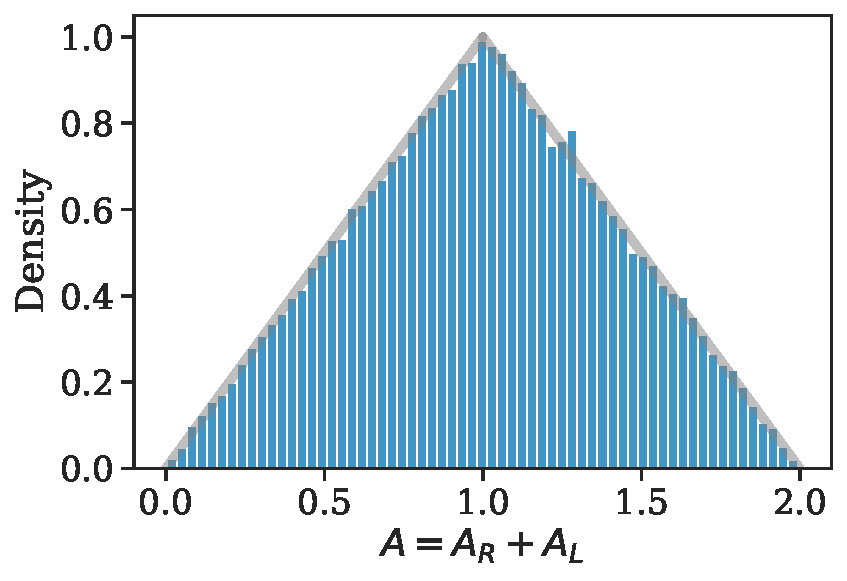
\includegraphics[width=\columnwidth]{jac_Aellip_RL}
\caption{Distribution imposed on the overall mode amplitude $A$ of Eq.~\eqref{eq:ellip} by assuming a uniform prior on the circular mode amplitudes $A_R, A_L$ in the range $[0, 1]$.}
\label{fig:jac_rl}
\end{figure}

% \begin{align}
% h_+ - i h_\times = C_{R}\, e^{-i \left(\omega t - \phi_R \right) } = C_R \cos(\omega t - \phi_R) - i \sin(\omega t - \phi_R)
% \end{align}

\subsection{Linear components}

Rather than using the circular basis, we could instead work with the linear polarization modes as the fundamental quantity and parametrize it as
\begin{subequations} \label{eq:Aphi}
\begin{equation}
h_+ = A_+ \cos (\omega t - \phi_+)\, ,
\end{equation}
\begin{equation}
h_\times = A_\times \cos (\omega t - \phi_\times) \, ,
\end{equation}
\end{subequations}
where $A_{+/\times}$ and $\phi_{+\times}$ are initial amplitudes and phases for each polarization.
Structurally, this mimics the parametrization adopted by \textsc{BayesWave} \cite{Cornish:2020dwh}, with the replacement $A_{+/\times} \to A_{+/\times} \exp\left(-t^2/\tau^2\right)$ and $\phi_{+/\times} \to -\phi_{+/\times}$ for some characteristic time $\tau$ for each wavelet.

\newcommand{\xp}{x_{+}}
\newcommand{\xc}{x_{\times}}
\newcommand{\xpc}{x_{+/\times}}
\newcommand{\yp}{y_{+}}
\newcommand{\yc}{y_{\times}}
\newcommand{\ypc}{y_{+/\times}}

% \newcommand{\xp}{A_{+,c}}
% \newcommand{\xc}{A_{\times,c}}
% \newcommand{\xpc}{A_{+/\times,c}}
% \newcommand{\yp}{A_{+,s}}
% \newcommand{\yc}{A_{\times,s}}
% \newcommand{\ypc}{A_{+/\times,s}}

The above equations also represent an elliptically polarized mode, albeit in a different parametrization than Eq.~\eqref{eq:ellip}.
To see this, first note that we can map Eq.~\eqref{eq:Aphi} into the circular-basis parameters of the previous section through the transformation
\begin{equation} \label{eq:Aphi_to_Cphi}
\begin{cases}
A_R = \frac{1}{2}\sqrt{A_+^2 + A_\times^2 + 2 A_+ A_\times \sin(\phi_\times - \phi_+)} \\
A_L = \frac{1}{2}\sqrt{A_+^2 + A_\times^2 - 2 A_+ A_\times \sin(\phi_\times - \phi_+)} \\
\phi_R = \mathrm{atan2}\left(\yp -\xc, \xp + \yc \right) \\
\phi_L = \mathrm{atan2}\left(-\yp -\xc, \xp - \yc \right)\, 
\end{cases} ,
\end{equation}
where, to simplify the notation, we have defined the cosine and sine quadratures
\begin{subequations} \label{eq:xy}
\begin{equation}
\xpc \equiv A_{+/\times} \cos \phi_{+/\times} \, ,
\end{equation}
\begin{equation}
\ypc \equiv A_{+/\times} \sin \phi_{+/\times} \, .
\end{equation}
\end{subequations}
Together with Eq.~\eqref{eq:Cphi_to_Aellip}, this allows us to compute $\{A, \epsilon, \theta, \phi\}$ as a function of $\{A_+, A_\times, \phi_+, \phi_\times\}$.
This transformation is clearly less straightforward than those for the circular components in the previous section, with amplitude and phase parameters mixing into each other.
This is because this coordinate transformation encodes the frame rotation that would bring an arbitrarily-oriented elliptical wave into the simple form of Eq.~\eqref{eq:Aphi}, which is nothing but the special frame we identified in Eq.~\eqref{eq:ellip_frame}.

\begin{figure}
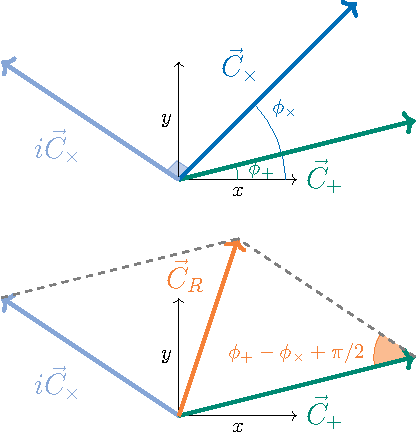
\includegraphics[width=0.8\columnwidth]{diagram_apac}
\caption{Geometric derivation of Eq.~\eqref{eq:Aphi_to_Cphi} for the right-handed polarization case.
\emph{Top:} Following Eq.~\eqref{eq:Aphi}, at time $t=0$, the plus and cross phasors, $\vec{A}_{+/\times} = A_{+/\times} \exp(-i \phi_{+/\times})$, subtend angles $-\phi_{+/\times}$ relative to the real axis ($x$, abscissa) and thus have Cartesian coordinates $\left(\xpc, - \ypc \right)$, in terms of the quantities defined in Eq.~\eqref{eq:xy}; the phasor $i\vec{A}_\times$ lies at a right angle from $\vec{A}_\times$, so that it subtends an angle $\pi/2 - \phi_\times$ with respect to the $x$-axis.
\emph{Bottom:} the right-handed phasor, $\vec{A}_R = \vec{A}_+ + i \vec{A}_\times$, has components $\left(\xp + \yc, -\yc - \xc\right)$ and, therefore, $\phi_R = \mathrm{atan2}( -\yc - \xc, \xp + \yc)$; since the acute angle between $\vec{A}_+$ and $i\vec{A}_\times$ is $\pi - (\pi /2 - \phi_\times) - \phi_+ = \phi_\times - \phi_+ + \pi/2$, the law of cosine implies $A_R^2 = A_+^2 + A_\times^2 + 2 A_+ A_\times \sin(\phi_\times - \phi_+)$.
This explains Eq.~\eqref{eq:Aphi_to_Cphi} for the right-handed case (the left-handed one is analogous).
}
\label{fig:diag_apac}
\end{figure}

We can gain some intuition for Eq.~\eqref{eq:Aphi_to_Cphi} by considering the relationship between the phasors associated with either the linear or circular polarizations (Fig.~\ref{fig:diag_apac}).
At any given time, interpret Eq.~\eqref{eq:Aphi} as the real parts of two complex numbers, such that
\beq
h_{+/\times} = \Re \left\{ A_{+/\times} \exp[-i\left(\omega t - \phi_{+/\times}\right)] \right\} .
\eeq 
Geometrically, this corresponds to vectors $\vec{A}_{+/\times}$ of magnitude $A_{+/\times}$, subtending angles $\phi_{+/\times} - \omega t$ with respect to the real axis.
At time $t=0$, then, the two linear polarizations lie at angles $\phi_{+/\times}$ away from the real axis; equivalently, in terms of the Cartesian components of Eq.~\eqref{eq:xy}, $\vec{A}_{+/\times} = \left(\xpc, - \ypc \right)$.
The initial state of the right- or left-handed circular polarizations can be similarly represented by phasors $\vec{A}_{R/L}$, related to the linear basis by the definition $h_{R/L} = h_+ \pm i h_\times$ (and hence $\vec{A}_R = \vec{A}_+ \pm i \vec{A}_\times$).
Using the fact that multiplication by $i$ is equivalent to a rotation by $\pi/2$ in the complex plane, it is straightforward to show that $\vec{A}_{R/L} = \left(\xp \pm \yc, -\yc \mp \xc\right)$, with the top (bottom) signs for R (L).
Equation~\eqref{eq:Aphi_to_Cphi} then follows trivially from the law of cosines, as illustrated in Fig.~\ref{fig:diag_apac}.

% \mi{I'm not sure this discussion actually helps build any intuition}
% To build some intuition for the above transformation, begin with Eq.~\eqref{eq:Cphi} and rearrange it using basic trigonometric identities to obtain
% \begin{widetext}
% \begin{align} \label{eq:Cphi_interm}
% h_+ - ih_\times &= A_{R}\, e^{-i \left(\omega t - \phi_R \right) } + A_{L}\, e^{i \left(\omega t + \phi_L \right) } \nonumber \\
% &= \left[A_R \cos(\omega t - \phi_R) + A_L \cos(\omega t - \phi_L)\right] - i\left[ A_R \sin (\omega t - \phi_R) - A_L \sin(\omega t - \phi_L)\right]  \nonumber \\
% &= \left[\cos\omega t \left( A_R \cos \phi_R + A_L \cos \phi_L \right) + \sin \omega t \left(A_R \sin \phi_R - A_L \sin \phi_L \right) \right] \nonumber \\
% &\phantom{=} - i \left[\cos\omega t \left(-A_R \sin\phi_R - A_L \sin\phi_L\right) + \sin \omega t \left( A_R \cos\phi_R - A_L \cos\phi_L\right)\right] .
% %&= \left(\xp \cos\omega t + \yp \sin\omega t\right) - i \left(\xc \cos\omega t + \yc \sin\omega t\right)
% \end{align}
% \end{widetext}
% Now note that Eq.~\eqref{eq:Aphi} and the definitions in Eq.~\eqref{eq:xy} imply
% \begin{align}
% h_+ - i h_\times &= \left(\xp \cos\omega t + \yp \sin\omega t\right) \nonumber\\
% &\phantom{=}- i \left(\xc \cos\omega t + \yc \sin\omega t\right) .
% \end{align}
% By direct comparison with Eq.~\eqref{eq:Cphi_interm}, we must then have
% \begin{equation}
% \begin{cases}
% \xp = A_R \cos\phi_R + A_L \cos \phi_L \\
% \yp = A_R \sin\phi_R - A_L \sin \phi_L \\
% \xc = -A_R \sin\phi_R - A_L \sin \phi_L \\
% \yc = A_R \cos\phi_R - A_L \cos \phi_L \\
% \end{cases},
% \end{equation}
% from which Eq.~\eqref{eq:Aphi_to_Cphi} follows after some manipulation taking advantage of the inverse of Eq.~\eqref{eq:xy}, namely
% \begin{subequations}
% \begin{equation}
% A_{+/\times} = \sqrt{\xpc^2 + \ypc^2} \, ,
% \end{equation}
% \begin{equation}
% \phi_{+/\times} = \mathrm{atan2}\left(\ypc, \xpc\right) .
% \end{equation}
% \end{subequations}

The overall Jacobian relating $\{A, \epsilon, \theta, \phi\}$ to $\{A_+, A_\times, \phi_+, \phi_\times\}$ is quite simple when expressed in terms of the first set of parameters,
\begin{subequations} \label{eq:jac_Aphi}
\begin{align}
J_2 &\equiv \left| \frac{\partial(A, \epsilon, \theta, \phi)}{\partial(A_+, A_\times, \phi_+, \phi_\times)}\right| \nonumber \\
&= 2 A_+ A_\times/ \left[ \sqrt{A_+^4 + A_\times^4 + 2 A_+^2 A_\times^2 \cos 2(\phi_\times - \phi_+)} \right. \nonumber \\
& \times \left( \sqrt{A_+^2 + A_\times^2 -2 A_+ A_\times \sin(\phi_\times-\phi_+)} \right. \nonumber \\
&\left.\left. +  \sqrt{A_+^2 + A_\times^2 +2 A_+ A_\times \sin(\phi_\times-\phi_+)}\right)\right]\\
&= \frac{1}{2 A} \sqrt{\left(\frac{1 + \epsilon^2}{1 - \epsilon^2}\right)^2 - \cos^2 2\theta} \, .
\end{align}
\end{subequations}
The $J_2 \propto 1/A$ dependence of this Jacobian implies that an analysis with uniform priors on the $\{A_+, A_\times, \phi_+, \phi_\times\}$ quantities will implicitly favor high signal amplitudes.
Additionally, Fig.~\ref{fig:jac_Aphi} shows the dependence of this Jacobian as a function of $\epsilon$ and $\theta$ for a fixed (nonzero) value of $A$.
The Jacobian diverges to positive infinity for $\epsilon = \pm 1$, meaning that purely circular polarizations will be heavily disfavored if we apply uniform priors on the $\{A_+, A_\times, \phi_+, \phi_\times\}$ quantities.

\begin{figure}
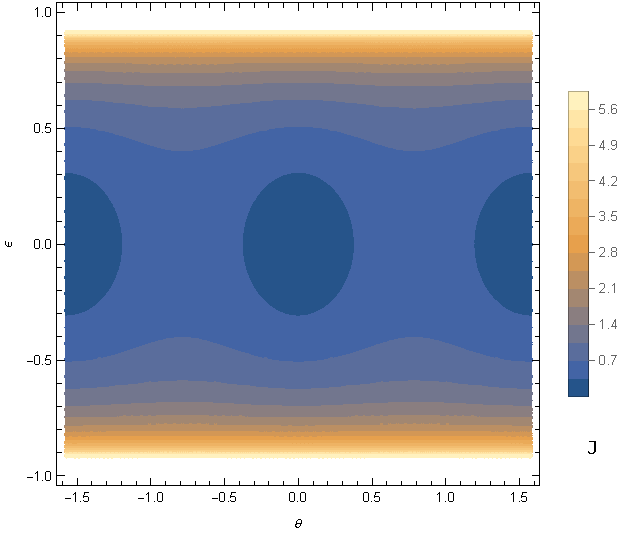
\includegraphics[width=\columnwidth]{jac_Aellip_Aphi}
\caption{Contour levels for the Jacobian relating the $\{A, \epsilon, \theta, \phi\}$ and $\{A_+, A_\times, \phi_+, \phi_\times\}$ parametrizations, Eq.~\eqref{eq:jac_Aphi}, as a function of the wave ellipticity $\epsilon$ and ellipse-orientation angle $\theta$ for a fixed value of $A$.}
\label{fig:jac_Aphi}
\end{figure}

\begin{figure*}
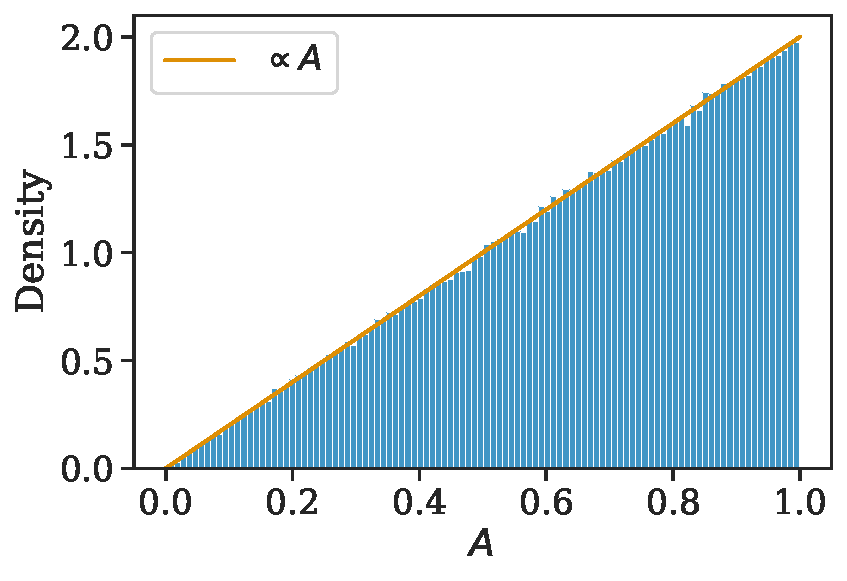
\includegraphics[width=\columnwidth]{jac_Aellip_Aphi_A}
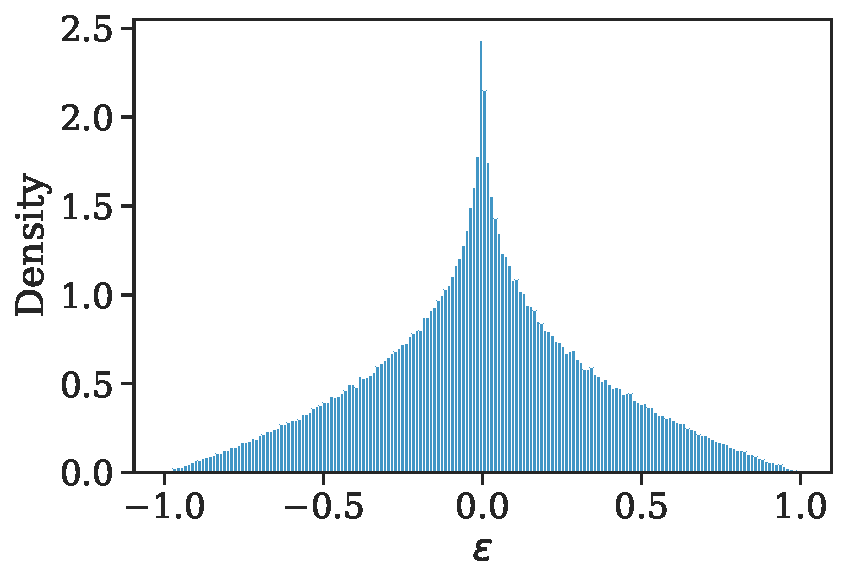
\includegraphics[width=\columnwidth]{jac_Aellip_Aphi_epsilon}\\
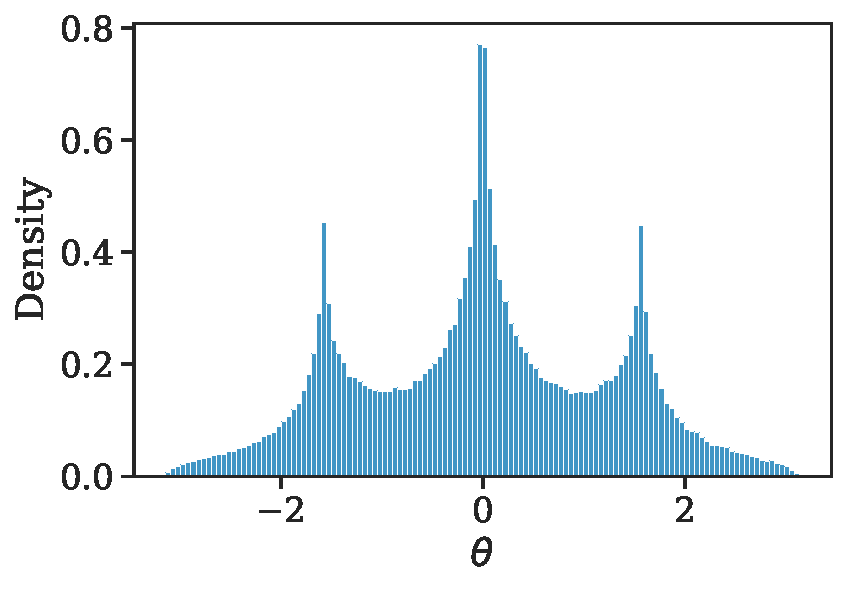
\includegraphics[width=\columnwidth]{jac_Aellip_Aphi_theta}
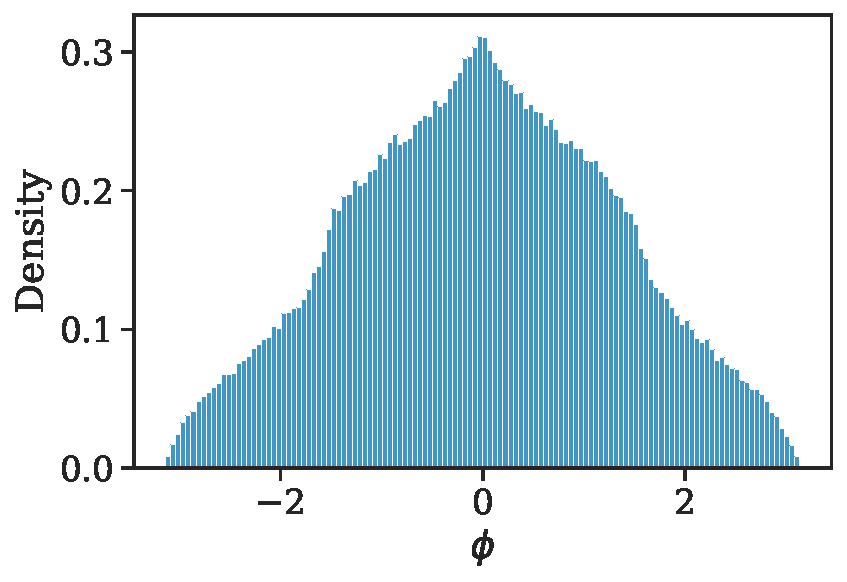
\includegraphics[width=\columnwidth]{jac_Aellip_Aphi_phi}
\caption{Marginal distributions imposed on the polarization ellipse parameters $\{A, \epsilon, \theta, \phi\}$ of Fig.~\ref{fig:ellipse} by drawing uniformly in the linear polarization parameters $\{A_+, A_\times, \phi_+, \phi_\times\}$ parameters of Eq.~\eqref{eq:Aphi} from $0\leq A_{+/\times} \leq 1$ and $0 \leq \phi_{+/\times} \leq 2\pi$, and constraining to $A \leq 1$.
The resulting distribution is favors large amplitudes (top left), favors linear polarizations (top right), and is anisotropic (bottom row).
}
\label{fig:jac_Aphi_pars}
\end{figure*}

That is indeed the behavior we find in Fig.~\ref{fig:jac_Aphi_pars} when sampling uniformly from $0\leq A_{+/\times} \leq 1$ and $0 \leq \phi_{+/\times} \leq 2\pi$, with an additional constraint that $A \leq 1$ for the resulting overall signal amplitude.
Enforcing this extra condition ensures that isotropy is preserved for the cosine and sine quadratures of the $+$ and $\times$ polarizations (we return to this below).

The strong preference for 

\subsection{Linear polarization quadratures}

Instead, it can be helpful to sample in terms of the cosine and sine quadratures corresponding to the polarizations of Eq.~\eqref{eq:ellip}.

\begin{equation}
h_+ = A_{+,c} \cos \omega t + A_{+,s} \sin \omega t
\end{equation}
\begin{equation}
h_\times = A_{\times,c} \cos \omega t + A_{\times,s} \sin \omega t
\end{equation}

\section{Nontensor polarizations}
\label{sec:nongr}

\newcommand{\xsym}{\ensuremath{\rm x}}
\newcommand{\ysym}{{\rm y}}
\newcommand{\bsym}{{\rm b}}
\newcommand{\lsym}{{\rm l}}
\newcommand{\hx}{h_{\xsym}}
\newcommand{\hy}{h_{\ysym}}
\newcommand{\hb}{h_{\bsym}}
\newcommand{\hlon}{h_{\lsym}}

Metric theories beyond GR may allow up to six independent polarizations, including the two tensor $+$ and $\times$ modes expected in GR.
The discussion above generalizes easily to include those additional modes, starting with an enhanced version of the driving matrix in Eq.~\eqref{eq:hij},
\beq \label{eq:hij_ngr}
(h_{ij}) = \begin{pmatrix}
\hb + h_+ & h_\times  & \hx  \\
h_\times  & \hb - h_+ & \hy  \\
\hx    & \hy    & \hlon
\end{pmatrix} ,
\eeq
where, in addition to plus and cross, also appear the vector-$x$ (\xsym) and vector-$y$ modes (\ysym), as well as the scalar breathing (\bsym) and longitudinal (\lsym) modes.%
\footnote{There are other possible normalizations in use in the literature, e.g., $\hlon \to \sqrt{2} \hlon$.}
Equivalently, as above, we can write this as a weighted sum over polarization tensors,
\beq
h_{ij} = \sum_p h_p\, e^p_{ij} \, ,
\eeq
for $p$ in $\{+,\times, \xsym, \ysym, \bsym, \lsym\}$, and polarization tensors $e^p_{ij}$ defined implicitly by comparison with Eq.~\eqref{eq:hij_ngr}.
Generally, the $h_p$ are functions of time, as for plus and cross above.

The considerations presented above regarding wave frame orientation and antenna pattern symmetries apply just as well to the generalized polarization tensor of Eq.~\eqref{eq:hij_ngr}, except for the different properties that the beyond-GR modes exhibit under rotations.
A rotation by $\Delta \psi$ around the line of propagation transforms the two vector amplitudes by
\begin{subequations} \label{eq:htransf_v}
\beq
\hx \rightarrow \hx' = \hx \cos \Delta \psi - \hy \sin \Delta\psi \, ,
\eeq
\beq
\hy \rightarrow \hy' = \hx \cos \Delta \psi + \hy \sin \Delta\psi \, ,
\eeq
\end{subequations}
reflecting the fact that these are the components of a spin-weight $s=1$ field (hence ``vector'').
On the other hand, the two scalar modes are invariant under rotations around $z$,
\begin{subequations} \label{eq:htransf_s}
\beq
\hb \rightarrow \hb' = \hb\, ,
\eeq
\beq
\hlon \rightarrow \hlon' = \hlon\, ,
\eeq
\end{subequations}
revealing that these behave as spin-weight $s=0$ fields (hence ``scalar'').

With similar assumptions as in the GR case, the detector output can be written as a sum over polarizations weighted by antenna patterns,
\beq \label{eq:h_ngr}
h(t) = \sum_p F_p(\alpha, \delta; \psi)\, h_p(t)\, ,
\eeq
with $F_p \equiv D^{ij} e^p_{ij}$ as before. 

As it turns out, differential-arm GW detectors are only sensitive to the traceless linear combination of the two scalar polarizations.
In terms of the breathing and longitudinal modes above, this is
\beq
h_{\rm s} \equiv \hb - 2\hlon\, ,
\eeq
which is the only scalar mode measurable by existing detectors.
Equivalently, the antenna patterns for the breathing and longitudinal modes are the same up to an overall constant (with our normalization, $F_{\bsym} = -F_{\lsym}$).
Therefore, the two terms are degenerate in Eq.~\eqref{eq:h_ngr} and their contributions cannot be disentangled in a model-independent way, i.e., without theory- and source-specific information about the specific morphology of the $\hb(t)$ and $\hlon(t)$ functions.
For unmodeled analyses, it thus suffices to include only one scalar term in Eq.~\eqref{eq:h_ngr}---commonly that for the breathing mode---so that the sum is over only five polarizations instead of six.

\section{Conclusion}

\begin{acknowledgments}
% NASA
M.I.\ is supported by NASA through the NASA Hubble Fellowship
grant No.\ HST-HF2-51410.001-A awarded by the Space Telescope
Science Institute, which is operated by the Association of Universities
for Research in Astronomy, Inc., for NASA, under contract NAS5-26555.
% % LIGO
% M.I.\ is a member of the LIGO Laboratory.
% LIGO was constructed by the California Institute of Technology and
% Massachusetts Institute of Technology with funding from the National
% Science Foundation and operates under cooperative agreement PHY-0757058.
% DCC
This paper carries LIGO document number \dcc{}.
\end{acknowledgments}

% \appendix

% \section{Circular Fourier amplitudes}
% \label{app:circ}
% 
% Here we fill in the steps relating the circular polarization Fourier amplitudes, $\tilde{h}_{R/L}$, to the Fourier amplitudes of the complex strain, $\tilde{H}$, as introduced in Sec.~\ref{sec:ellip}.
% Begin with the expression for the time-domain strain in terms of the linear components, Eq.~\eqref{eq:planewave},
% \begin{align}
% h_{ij}(t) &= \int_{-\infty}^{+\infty} \left[\tilde{h}_+(\omega) e^+_{ij} + \tilde{h}_\times(\omega) e^\times_{ij}\right] e^{-i\omega t} \infd \omega \nonumber\\ 
% &=\left[\int\tilde{h}_+e^{-i\omega t} \infd \omega\right] \hspace{-2pt} e^+_{ij} + \left[\int \tilde{h}_\times e^{-i\omega t} \infd \omega\right] \hspace{-2pt} e^\times_{ij},
% \end{align}
% where we have suppressed limits of integration and $\omega$ dependence when obvious.
% %
% Picking out the $h_{+/\times}$ amplitudes from $h_{ij} = h_+ e^+_{ij} + h_\times e^\times_{ij}$, the complex strain can then be written as
% %\begin{widetext}
% \begin{align}
% h_+ - i h_\times &= \int\tilde{h}_+e^{-i\omega t} \infd \omega -i \int \tilde{h}_\times e^{-i\omega t} \infd \omega \nonumber \\
% &= \int \left(\tilde{h}_+ -i \tilde{h}_\times \right) e^{-i\omega t} \infd \omega \nonumber \\
% &= \sqrt{2} \int_{-\infty}^{\infty} \tilde{h}_R(\omega)\, e^{-i\omega t} \infd \omega \, ,
% \end{align}
% where we have used the expression for $\tilde{h}_R$ in Eq.~\eqref{eq:circ_amps}.
% By direct comparison with Eq.~\eqref{eq:hcomp_fd}, it is now obvious that $\tilde{H}(\omega)= \sqrt{2} h_R(\omega)$.
% 
% Furthermore, we can take advantage of Eq.~\eqref{eq:sym_circular} to rewrite the above integral only in terms of positive frequencies as
% \begin{align}
% h_+ - i h_\times &= \sqrt{2}\int_{0}^{\infty} \left[\tilde{h}_R(\omega) e^{-i\omega t} + \tilde{h}_R(-\omega) e^{i\omega t} \right] \infd \omega \nonumber \\
% &= \sqrt{2}\int_{0}^{\infty} \left[ \tilde{h}_R(\omega) e^{-i\omega t}  + \tilde{h}^*_L(\omega) e^{i\omega t}\right] \infd \omega
% \end{align}
% %\end{widetext}
% so $H(\omega)= \sqrt{2} h_R(\omega)$ and $H_L = \sqrt{2} h_L^*$.


\bibliography{refs}

\end{document}
%
% ****** End of file apstemplate.tex ******
